\chapter{Lemmatisation}
\label{sec:lemmatiseurs}

\section{Introduction}
\label{subsec:lemma_intro}

Afin de traiter un texte et d'établir des statistiques sur celui-ci, il est courant de le lemmatiser. La lemmatisation d'un texte, et \textit{a fortiori} d'un mot, correspond à sa transformation en
%ou bien on "l'associe à"
une forme canonique, le \textit{lemme}. Traditionnellement identique à la forme d'entrée
%nope, le mot vedette
d'un dictionnaire, le lemme permet de rassembler sous une même étiquette l'ensemble des formes fléchies et variations graphiques qu'il peut connaître. Pour le latin, il s'agira de rassembler ensemble \textsc{me} et \textsc{mihi} sous une racine commune \textsc{ego}. Cet étiquetage permet de clarifier le signal statistique en éliminant où cela est nécessaire un bruit inhérent aux langues flexionnelles (voire aux langues dont le système graphique est variable, potentiellement influencé localement, comme l'ancien français ou le latin épigraphique). Son utilisation principale a longtemps eu pour but la capacité à trouver dans un texte les occurrences d'un terme puis a permis le développement plus tardivement de la linguistique de corpus\footcite{mellet2002atouts}.

\subsection{Tâches et définitions générales}

La lemmatisation est donc un effort de traduction d'un texte en un ensemble de formes normalisées, de telle façon qu'\textit{un mot} ne doit connaître qu'une seule annotation de lemme. Notre définition\footnote{On retrouve cette définition partagée par de nombreuses ressources, entre autres \textit{Wikipedia} anglais et français, et dans la plupart des articles et cours d'introduction à la lemmatisation récents. Par exemple, chez \textcite{srinidhi_lemmatization_2020}: \quote{\textit{Both in stemming and in lemmatization, we try to reduce a given word to its root word.}}} exclut \textit{ipso facto} les outils d'analyse du vocabulaire tels que \textit{Collatinus} qui propose pour chaque forme l'ensemble de possibilités de lemme qu'il estime compatible avec la forme. Ainsi, là où \textit{est} est identifié comme \textsc{edo} et \textsc{sum} par \textit{Collatinus}, un lemmatiseur fait un choix unique, lié généralement au contexte et à la probabilité afférente d'apparition de chacun des lemmes possibles à cet endroit.

Enfin, dans le cadre de la lemmatisation, on préfèrera l'utilisation du terme \enquote{\textit{token}} à celui de \enquote{mot}. En traitement automatique des langues, le \textit{token} est un élément dans un ensemble. Au niveau texte, on découpe volontiers ce dernier en séquences plus ou moins indépendantes, généralement des phrases pour les tâches qui nous préoccupent: ainsi, dans ``\textit{II mulieres Gallaeque estis. Romanus sum.}'', nous avons deux \textit{tokens}, ``\textit{II mulieres Gallaeque estis.'}' et ``\textit{Romanus sum.}''. Au niveau inférieur, dans ces unités longues indépendantes, le \textit{token} est un élément qui correspond à la fois aux mots (\textit{mulieri}), aux nombres (\textit{II}), aux enclitiques (\textit{-que}), mais aussi aux signes de ponctuation (\textit{.}). Pour le latin, la tokenisation cherchera donc potentiellement à extraire les enclitiques: \mintinline{python}{"Gallaeque"} se découpera ainsi en \mintinline{python}{["Gallae", "-que"]}\footnote{Cette tâche n'est pas aussi facile que pourrait le laisser deviner cet exemple: pour les lemmes en \textit{-o, -onis} de la troisième déclinaison, le choix entre une forme \textit{Observatione} découpée en \mintinline{python}{["Observatio", "-ne"]} ou conservée telle quel pour représenter un ablatif singulier ne peut se faire qu'en contexte.}. Ce travail est d'autant plus important qu'il peut faire une différence notable dans le cadre de l'annotation: ainsi, identifier \mintinline{python}{"P. Naso."} en un \textit{token} de premier niveau et trois \textit{tokens} de deuxième (une phrase, 3 éléments dont une abréviation, \mintinline{python}{["P.", "Naso", "."]}) plutôt qu'en deux de deux chacun (deux phrases de deux éléments chacune, \mintinline{python}{["P", ".", "Naso", "."]}) induira une rupture de syntaxe, un changement de contexte qui compliquerait la lemmatisation de \textit{Naso} par exemple en \textsc{nasus} le nez plutôt qu'en \textit{cognomen} \textsc{Naso}.


En plus de la lemmatisation, on trouve souvent adjointes deux types supplémentaires  relevant de l'annotation automatique (ou tâches) sur ces \textit{tokens}, basées sur des analyses syntaxiques ou morphosyntaxiques. D'une part, on retrouve très souvent l'annotation des \textit{Part-Of-Speech} (POS). Cette tâche est traitée très rapidement - dès les années 1990 - par les annotateurs automatiques tels que TreeTagger\footcite{schmid1994treetagger}. Les catégories de POS, que l'on pourrait traduire par la notion de nature en français, consistent en un ensemble de catégorisations grammaticales (et non sémantiques) dépendantes des distributions syntaxiques, des fonctions syntaxiques, et enfin des morphologies acceptables\footcite{schachter1985parts}. En traitement automatique du langage, qu'il s'agisse par exemple de stylométrie\footcite{Cafieroeaax5489}, de classification des genres de texte\footcite{feldman2009part}, ou enfin d'analyse de sentiments\footcite{wang2015pos}, les POS ont démontré un réel apport comme variable (\textit{feature}) des données d'entrées de modèles de prédiction. D'autre part, on pourra ajouter à l'annotation une information morphologique ou morphosyntaxique. Elle peut être prise comme un tout (féminin singulier) ou comme un ensemble d'informations indépendantes (féminin; singulier). On distinguera l'information purement morphologique, qui veut que \textit{bonum}, à l'accusatif est un masculin neutre, de l'information morphosyntaxique, qui veut que \textit{bonum virum} est un masculin. En latin, on compte 8 de ces catégories (Cas, Nombre, Genre, Degré, Mode, Temps, Voix, Personne), chacune avec ses valeurs particulières, et une catégorie supplémentaire en cas d'absence de l'ensemble de celle-ci, pour des termes sans morphologie, comme \enquote{ut}. L'usage de ces traits morphologiques comme \textit{features} n'est pas encore très étudié, %
% je crois 
mais on en trouve des exemples dans certaines études sur la reconnaissance d'entités nommées par exemple \footcite[Par exemple]{zirikly2014named}. Leur utilisation comme variable dans notre étude pourrait se révéler utile: en effet, l'intuition voudrait que l'identification des agents (via les cas et la voie des verbes en contexte), de leur genre et enfin les modes verbaux (l'impératif en particulier) puissent apporter des contributions importantes à la classification d'extraits sur le sujet de la sexualité.


\subsection{Une histoire riche, en particulier pour le latin}

La lemmatisation, en latin, possède une histoire particulièrement riche et liée à celle des humanités numériques \footnote{Une majorité des pistes de recherche nous est fournie par la présentation de N. Perreaux, \textit{cf.} \cite{perreaux_lemmatisation_2019}}. Il ne s'agira pas ici de faire une histoire exhaustive de la lemmatisation et de son application au latin, mais plutôt d'évoquer des continuités et des ruptures amenant à l'état que l'on connait aujourd'hui de la matière.

Il faut noter que les études classiques ont fait usage de la lemmatisation avant le passage à son usage informatique, à travers la création des index et en particulier, dans leur forme la plus ancienne, des concordanciers. M. et R. Rouse datent l'apparition de ces derniers dans leur forme plus ou moins actuelle au XIII\textsuperscript{e} siècle, à travers les trois concordances verbales de la Bible, à savoir, dans l'ordre chronologique\footcite{rouse_concordance_1984}: celle de Saint-Jacques (\textit{circa} 1235), la concordance anglaise (sans datation connue, sans exemplaire survivant) et une troisième concordance, qui ne saurait être rédigée après 1285. Les auteurs de cette histoire de la concordance attribuent par ailleurs l'apparition de cette forme non seulement au besoin d'enseigner et d'étudier les Écritures, mais aussi de rassembler une pratique apparaissant au cours du XII\textsuperscript{e} siècle de la \textit{concordantia}, qui consistait à adjoindre aux gloses les références d'autres passages de la Bible liés au terme glosé. Quoi qu'il en soit, il apparait dans ces concordances, comme dans les dictionnaires, une vedette (le lemme) avec l'ensemble de ces formes fléchies en contexte. Il faudra attendre le XIV\textsuperscript{e} siècle, puis le XV\textsuperscript{e} siècle pour qu'apparaissent deux autres concordances, l'une sur la Septante grecque, l'autre sur l'Ancien Testament hébreu.

\begin{figure}[h]
    \centering
    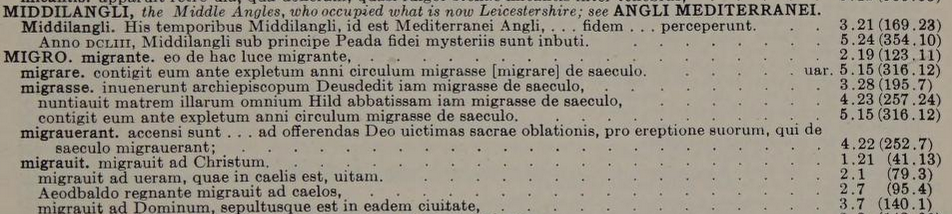
\includegraphics[width=\textwidth]{figures/chap3/JonesConcordance.png}
    \caption{Extrait de  \textit{A concordance to the Historia ecclesiastica of Bede} de Jones, Putnam Fennell.}
    \label{fig:chap3:concordance_jones}
\end{figure}

\begin{figure}[h]
    \centering
    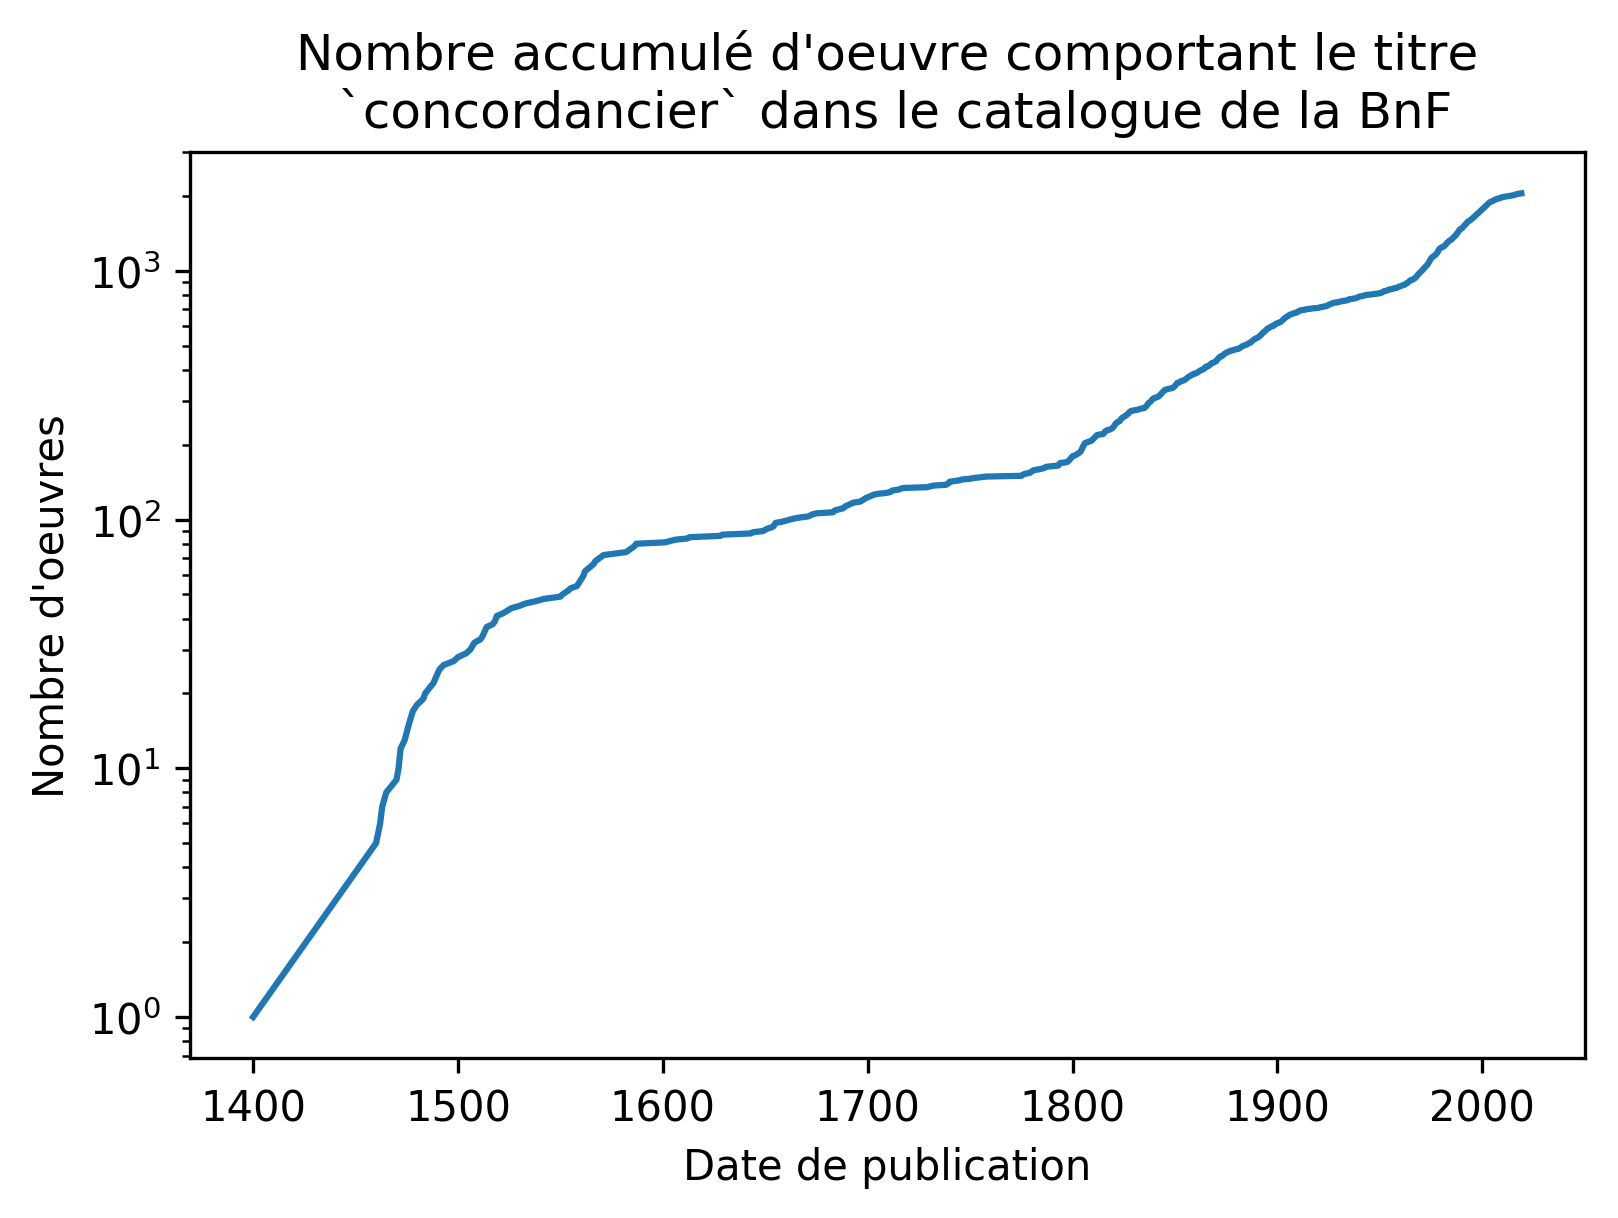
\includegraphics[width=10cm]{figures/chap3/histoire/concordanciers.png}
    \caption{Accumulation par dates de concordanciers conservés à la Bibliothèque Nationale de France d'après une recherche sur le catalogue général.}
    \label{lemmatisation:concordanciers}
\end{figure}

Et il ne s'agit pas que des concordances où le latin a été le premier à être lemmatisé de manière systématique pour une étude du langage. Dans le cadre du projet de Roberto Busa, à partir de 1949, on assiste à la première lemmatisation enregistrée numériquement (bien que sur des fiches perforées) via une collaboration avec IBM. Ce travail novateur aura pour but la constitution d'un corpus gigantesque de 11 millions de mots pour une publication vers 1980 de 56 volumes. Ce travail titanesque est d'ailleurs généralement vu comme l'un des projets fondateurs des humanités numériques: Roberto Busa est certainement aux humanités numériques ce que Thucydide et Hérodote sont à l'histoire, dans la méthode du premier comme dans le mythe personnel du second. Cette innovation mécanographique est inédite, mais ne connait pas d'impact direct et immédiat: il faut attendre les années 60 et une  croissance à la fois de l'accès à l'outil informatique (sans parler de démocratisation), de la linguistique de corpus et et de la statistique textuelle (entre autres assistée par ordinateur) pour qu'une suite, ou du moins une méthode parallèle, voit le jour. 

La première occurrence universitaire d'un travail systématique de lemmatisation apparait à l'université de Liège avec le travail du LASLA, fondé le 13 septembre 1961\footcite{delatte_laboratoire_1961}. Dans leur article inaugural, les auteurs Louis Delatte et Étienne Évrard traitent de l'importance de la statistique en matière d'études stylistiques, et, partant du constat que les indices à disposition des chercheurs sont \enquote{incomplets, inexacts ou même inexistants}, ils proposent un travail systématique d'annotation des textes latins et leur enregistrement mécanographique. Tout en portant de nombreuses critiques envers un possible manque de rigueur statistique de certains philologues, cet article montre surtout les opportunités, dans la continuité scientifique du domaine gréco-romain, que porterait un tel outil, à savoir l'assurance de détecter des phénomènes non pas subjectivement ou intuitivement, mais à partir de \enquote{comparaisons entre probabilités théoriques et fréquences réelles}. Par ailleurs, l'article annonce la première étape du laboratoire, à savoir l'annotation des œuvres de Sénèque. La perspective des deux fondateurs du laboratoire est révolutionnaire, et la violence à demi-voilée des propos \footnote{\enquote{Dans combien d'allitérations purement fortuites les commentateurs n'ont-ils pas voulu découvrir les intentions les plus subtiles}, \cite[p.~442]{delatte_laboratoire_1961}} rencontre très rapidement des phénomènes de résistance. Dans une perspective d'histoire du domaine de la lemmatisation, Nicolas Perraux\footcite{perreaux_lemmatisation_2019} a fait resurgir une polémique qui va en ce sens entre Pierre Grimal et Louis Delatte. Aux détours de quatre articles (\footcites{grimal_delatte_1964}{delatte_propos_1965}{grimal_index_1966}{delatte_index_1968}) dont deux sont des comptes-rendus, les deux philologues engagent une \enquote{guerre franco-belge}\footcite{verdiere_pierre_1970}, initiée par P. Grimal, tournant autour de trois points principaux:
\begin{itemize}
    \item Sans aucun doute, il y a ici une question de territoire intellectuel. Nous ne pouvons ignorer que P. Grimal tend à se positionner comme spécialiste francophone incontesté de Sénèque\footcite{verdiere_pierre_1970}, et, alors qu'il écrit une critique de l'index de L. Delatte publié en 1962, se prépare aussi à publier le sien. Dans le même contexte, quand L. Delatte fait une critique de la concordance de l'\textit{ad Marciam} de P. Grimal (publiée en 1965), il le fait aussi en défense de la publication de son propre index de 1964.
    \item De manière sûre et certaine, il y a un débat sur la question de la concordance, conservant le contexte, contre l'index, répertoriant uniquement les passages de chaque lemme. Cette question de la forme, en dehors de toute méthode, est par ailleurs ravivée en 1979, quand L. Delatte et deux collègues\footcite{delatte_concordantiae_1979} viennent critiquer la concordance de Sénèque, générée pourtant automatiquement via des fiches mécanographiques, éditée par Roberto Busa.
    \item Enfin, et c'est un problème clair, une résistance complète et totale à la question du numérique de la part de P. Grimal. L. Delatte pose cependant un ensemble de jalons importants pendant les années soixante, non seulement en créant la \textit{Revue de l'Organisation Internationale pour l'Étude des Langues Anciennes par Ordinateur} \footnote{Aujourd'hui nommée \textit{Revue du LASLA}. Autrefois abrégée RELO} mais en fondant sa pratique de la mécanographie sur un pilier simple, celui de tout enregistrer pour pouvoir manipuler, statistiquement ou traditionnellement, des données en séries: \enquote{Le document de travail est, pour nous, le fichier de cartes perforées}\footcite[p~.202]{delatte_index_1968}. Au contraire, P. Grimal se réfugie tour à tour derrière des considérations matérielles (\enquote{D’ailleurs, qui a son ordinateur personnel ?}\footcite[p.~111]{grimal_index_1966}) ou bien une incompréhension des possibilités de l'informatique:
\end{itemize}
    

\begin{quote}
    \blockquote{Renoncer à la machine, ce serait aussi se libérer d'un certain nombre de servitudes, comme l'adoption d'un code qui devient rapidement assez complexe lorsqu'on cherche à condenser un grand nombre de renseignements sur une fiche. La machine ne peut connaître que des catégories bien définies, chacune étant traduite par un symbole. Ces catégories constituent comme un quadrillage à l'intérieur duquel le réel doit entrer de gré ou de force, sans déborder d'une case dans l'autre\footcite[p.~131]{grimal_delatte_1964}}
\end{quote}

Quoi qu'il en soit, si cette polémique, s'étirant sur une dizaine d'années, entre Liège et Paris, nous montre des formes de résistances et des questions quant aux nouvelles formes qui émergent, elle fait aussi ressortir le travail titanesque qui se fait autour de L. Delatte et É. Évrard au LASLA. Il est y fait mention d'une \enquote{machine à lemmatiser} dès 1965\footcite{delatte_programme_1965} qui propose pour une forme donnée l'ensemble des lemmes pouvant s'y rattacher, faisant tourner des rouages algorithmiques autour de quatre sets de données: les formes irrégulières, complètes, ne permettant aucune reconnexion (\textit{e.g.} les formes de \textsc{sum} au présent); les radicaux; les terminaisons avec leurs codes morphologiques; les préfixes verbaux (\textsc{ad-sum} par exemple, afin de réduire la taille des calculs.). Cette base d'analyseur morphologique est la même que pour \textit{Words}\footcite{whitaker_words_1993}, \textit{Morpheus}\footcite{crane_generating_1991}, \textit{LEMLAT}\footcite{bozzi_lemlat_1992} ou encore \textit{Analysis}\footcite{ouvrard_analysis_1992} qui devient ensuite \textit{Collatinus}\footcite{ouvrard_collatinus_1999}. Tous ces outils apparaissent au début des années 90, et deux, \textit{Collatinus} et \textit{Words}, sont issus du travail de passionnés, l'un professeur de latin, Yves Ouvrard, et l'autre colonel de l'armée étatsunienne, William Whitaker\footnote{D'après sa nécrologie, il était en effet membre de la \textit{Defense Advanced Research Projects Agency} (DARPA), mais \textit{a priori} retraité au moment de la création de Words. \textcite{noauthor_william_nodate}}.

Cependant, si l'on retient pour lemmatiseur une définition stricte d'annotation d'une forme par un lemme, impliquant un choix en contexte donc, le premier lemmatiseur du latin vient bien plus tard. Et il ne s'agira pas d'un lemmatiseur du latin, mais bien d'un lemmatiseur généraliste: ce que Delatte estimait potentiellement impossible en 1968\footnote{\enquote{Un tel programme, supposant d'ailleurs une analyse conceptuelle, est très difficile sinon impossible à réaliser}, \cite[p.~100]{delatte_index_1968}}), l'augmentation des puissances de calcul et de mémoire vive des ordinateurs a permis de le faire. À partir des années 1990, on voit apparaître des lemmatiseurs prenant en compte le contexte dans le choix des lemmes pour les formes ambivalentes. %(Insertion études par collatinus du nombre de lemme possible par forme ?). 
Pour prendre en compte ce voisinage des mots analysés, on a généralement donné à ces outils des données d'entraînement permettant la reconnaissance de phénomènes lexicaux et on voit alors la naissance de corpus(\textit{cf.} chapitre 1). Parmi ces outils, TreeTagger a, semble-t-il, reçu les faveurs de la communauté des latinistes des périodes classiques et médiévales, bien qu'il ne soit \textit{a priori} pas le plus performant\footcite[Voir]{eger_lexicon-assisted_2015}. Plusieurs hypothèses peuvent être émises quant à cette situation\footnote{Il faudrait, à ce sujet, probablement faire des recherches et des entretiens plus poussés que ne nous le permet notre sujet ici.}. Il se pourrait que les phénomènes suivants aient fortement influencé sa place actuelle dans le domaine: son incorporation via \textit{TXM}\footcite{heiden:halshs-00549779}, sa prise en main relativement tôt due à son ainesse de presque 10 ans sur certains autres taggers, sa facilité d'installation, la constitution de modèles relativement tôt. 


\begin{figure}[h]
    \centering
    \resizebox{\textwidth}{!}{%
    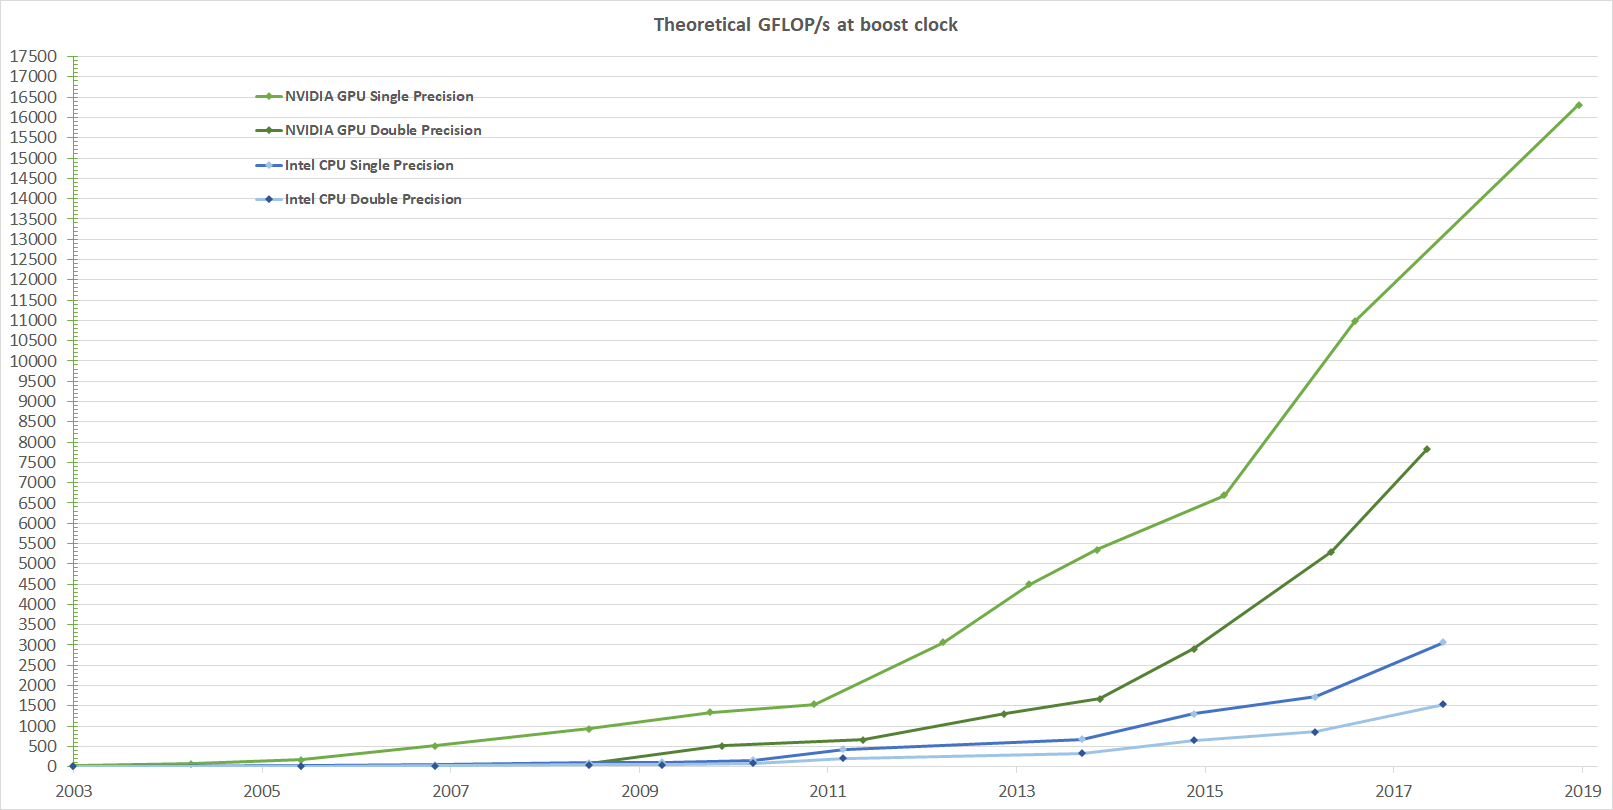
\includegraphics{figures/chap3/histoire/floating-point-operations-per-second.png}%
    }
    \caption{Opération à virgule flottante par seconde (FLOPS) entre processeur traditionnel (CPU) et de carte graphique (GPU). Source: \cite{noauthor_cuda_nodate}}
    \label{lemmatisation:histoire:puissance-gpu}
\end{figure}


Ces lemmatiseurs font face ensuite aux modèles complexes de \textit{deep learning} qui apparaissent au milieu et à la fin des années 2010, grâce à une montée en puissance continue des machines en calcul. En effet, dans un contexte d'amélioration des performances des cartes graphiques et de leurs GPUs (\textit{Graphical Processing Unit}, \textit{cf.} \ref{lemmatisation:histoire:puissance-gpu}), principalement poussée par une consommation en jeux vidéo du grand public\footcite{tanz_how_2017}, les chercheurs ont pu accéder à des machines beaucoup plus puissantes qu'auparavant pour des prix beaucoup plus faibles. En avril 2020, le prix d'une carte graphique professionnelle haut de gamme coûtait encore 7~602€ \footcite{noauthor_pny_2020} contre des prix variant de 1~149 à 1~899€ suivant les marques pour le haut de gamme à destination des particuliers\footcite{noauthor_recherche_2020}\footnote{C'est sur ce modèle que l'ensemble des entraînements de cette thèse a été produit.}, en septembre 2020, ce coût était encore potentiellement divisé par deux chez le même constructeur avec l'arrivée d'une nouvelle génération de cartes graphiques. Cette explosion de puissance et sa démocratisation permettent à de plus en plus de laboratoires de s'équiper, y compris ceux ne relevant pas du domaine des sciences de l'informatique, et aux chercheurs de prototyper de nouveaux modèles, permettant d'obtenir des temps d'entraînement particulièrement réduits\footnote{La très grande majorité des calculs se faisant via opération sur décimaux qui sont plus faciles pour les GPU que les processeurs classiques} et donc d'essayer un plus grand nombre de combinaisons possibles de modèles (en 2017, d'après \ref{lemmatisation:histoire:puissance-gpu}, la différence de puissance est de x4). Parallèlement à cette évolution du matériel, les géants du web investissent dans des librairies de développement telles que \textit{PyTorch} (Facebook) et \textit{Tensorflow} (Google) qui permettent elles aussi de faciliter le prototypage de modèles de prédiction sans avoir à gérer la réimplémentation de modèles mathématiques complexes inhérents à l'apprentissage profond. Ce contexte riche de démocratisation logicielle et matérielle permet à des projets comme Pandora \footcites{kestemont_lemmatization_2017}{de_gussem_integrated_2017} puis Pie\footcite{manjavacas_improving_2019} de naître dans des laboratoires non-spécialistes. 

\section{Les différents types d'outil}

\subsection{Les outils à base de règles (dès 1965)}

Dès 1965 et la création du LASLA donc, L. Delatte et É. Evrard cherchent à automatiser, en partie, la lemmatisation et l'annotation morphologique. Ce système semi-automatique, qui vise à proposer des solutions sans y faire un choix, repose sur l'utilisation de plusieurs bases de données (lexicales, morphologiques, affixales, etc.). Ce système fondé sur des bases de connaissances se retrouvent chez quatre autres outils cités plus haut, à savoir \textit{Words} de W. Whitaker, \textit{Morpheus} de G. R. Crane, \textit{Collatinus} de Y. Ouvrard (puis Philippe Verkerk à partir de 2015) ou encore, parmi les plus récents, \textit{LemLat}. À partir d'une base de lemmes, reliée à des bases de radicaux et de flexions, l'outil tente différentes combinaisons pouvant correspondre à la forme analysée: lorsqu'un radical et une flexion acceptée par ce radical s'accordent, un lemme et ses analyses morphologiques sont donnés (\textit{cf.} \ref{lemmatisation:outils:collatinusAlgorythme} et \ref{lemmatisation:outils:collatinusAlgorythme} pour des exemples basés sur Collatinus). Chacun de ces lemmatiseurs est basé sur un dictionnaire différent, faisant état de traditions philologiques propres à des centres de recherche ou à des systèmes éducatifs. En effet, \textit{Word} utilise l'\textit{Oxford Latin Dictionary}, \textit{Morpheus} utilise le \textit{Lewis \& Short}, le LASLA utilise le \textit{Forcellini}, Y. Ouvrard semble utiliser le \textit{Gaffiot}, \textit{LemLat} utilise principalement le \textit{Georges}. Cette différence pose un problème d'incompatibilité des différents outils. C'est d'ailleurs dans ce cadre que l'ERC LILA s'inscrit en tentant de proposer une réconciliation des différents référentiels de lemmes\footcite{mambrini_harmonizing_2019}. Dans cette catégorie d'outils rentrent aussi les outils à base de dictionnaire de formes comme celui du CLTK\footcite{johnson2014cltk} qui enregistrent pour chaque forme connue les lemmes et les analyses possibles, sans nécessairement chercher l'exhaustivité, et proposent les lemmes correspondant aux formes enregistrées.

\begin{figure}[h]
    \centering
    \resizebox{\textwidth}{!}{%
    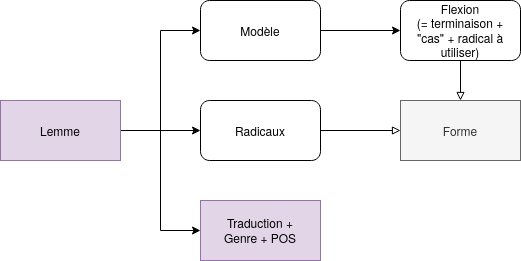
\includegraphics{figures/chap3/outils/CollatinusDB.png}%
    }
    \caption{Modèles de données dans Collatinus. Les formes sont générées et analysées à partir des flexions et radicaux, en fonction du modèle. }
    \label{lemmatisation:outils:collatinusDB}
\end{figure}


\begin{figure}[h]
    \centering
    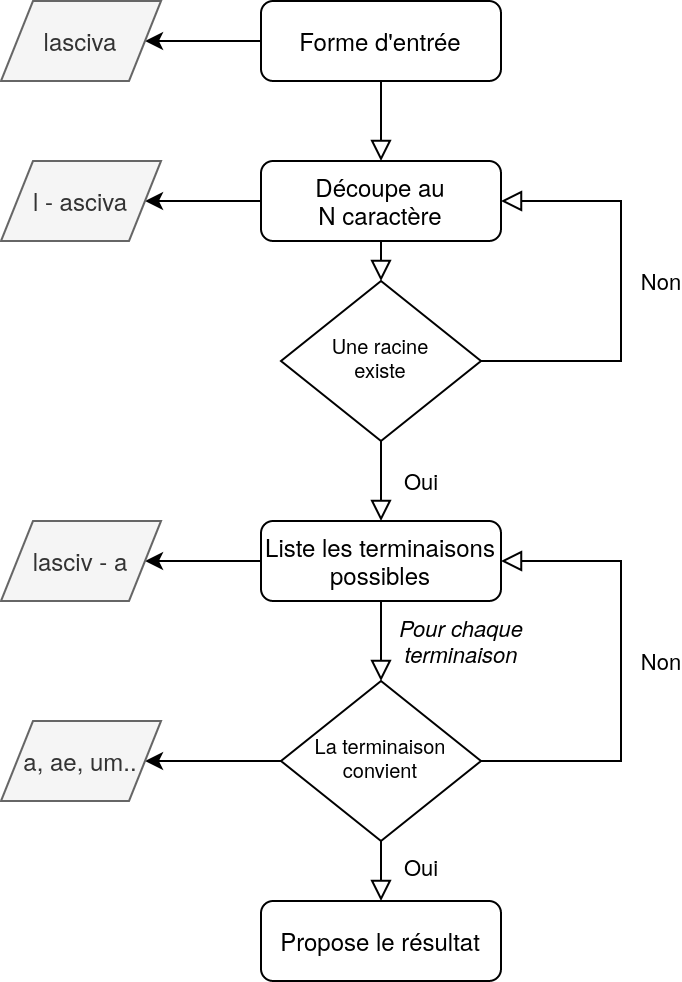
\includegraphics[width=6cm]{figures/chap3/outils/collatinus.png}
    \caption{Algorithme simplifié de Collatinus}
    \label{lemmatisation:outils:collatinusAlgorythme}
\end{figure}

L'avantage principal de ce type d'outils consiste en sa capacité d'ingérer de nouveaux lemmes très facilement. Par exemple, dans Collatinus, \textsc{lascivus} est donné par la ligne \texttt{lascīvus=lāscīvus|doctus|||a, um} où \texttt{a, um} est fourni dans un but lexicographique, mais n'a aucune utilité pour la génération des formes: seul \enquote{\textit{lascivus}} et \enquote{\textit{doctus}} (le modèle de déclinaison) suffisent pour cette partie de l'algorithme. Ainsi, pour ajouter un lemme \textsc{christianus}, au cas où ce lemme tardif n'était pas inscrit dans le \textit{Gaffiot} et donc dans \textit{Collatinus}, il suffirait d'ajouter, scansion omise, \texttt{christianus|doctus|||a, um}. À partir de ce simple ajout, la forme \textit{christiani} serait nécessairement reconnue. Le désavantage de ces outils réside dans leur incapacité à faire le choix dans les analyses possibles, qu'il s'agisse des analyses morphologiques (\textit{lasciva} est-il un nominatif singulier féminin ou un pluriel neutre ?) ou des choix de lemmes (\textit{ita} est-il un adverbe ou la deuxième personne du singulier présent impératif actif de \textsc{ito}).

\subsection{Les outils sur base statistique (1994 et après)}

Au milieu des années 90, mais surtout au début des années 2000 apparaissent les lemmatiseurs et analyseurs de POS tels que \textit{TreeTagger}\footcite{schmid1994treetagger}, mais aussi \textit{TnT}\footcite{brants_tnt_2000} et \textit{StanfordNLP}\footcite{toutanova_feature-rich_2003}. Leurs modèles sont principalement basés sur des structures à base de probabilités d'occurrences de phénomènes en contexte, en intégrant la POS à l'analyse de lemme: on parle d'ailleurs principalement de POS-Tagger pour ces outils. Pour faire simple, ces analyseurs font usage de dictionnaires avec des fréquences possibles de POS, puis, en fonction d'une séquence de quelques mots (3 ou 4 en général), telle que \enquote{\textit{fortissimi sunt Belgae}} pour \enquote{\textit{Horum omnium fortissimi sunt Belgae}}, ils cherchent à établir l'analyse plus probable, avec des stratégies de décisions et d'éliminations diverses. \textit{TreeTagger} change la donne en 1994 en apportant plusieurs modifications, qui probablement expliquent ses performances sur le latin. D'une part, il constitue un dictionnaire de suffixes en plus du dictionnaire de forme, d'autre part, pour faire face aux \enquote{\textit{ungrammaticalities}}\footcite[p.~2]{schmid1994treetagger} possibles de l'anglais, il attribue une probabilité minimale aux probabilités nulles\footnote{Il n'exclut pas les phénomènes improbables, en corrigeant les probabilités de 0 à 0,00001 par exemple.}. Dans le contexte d'une langue latine à l'ordre des mots non fixe et à la morphologie riche, ces deux facteurs pourraient expliquer une augmentation des scores importants comparés aux modèles précédents.

\begin{figure}[h]
    \centering
    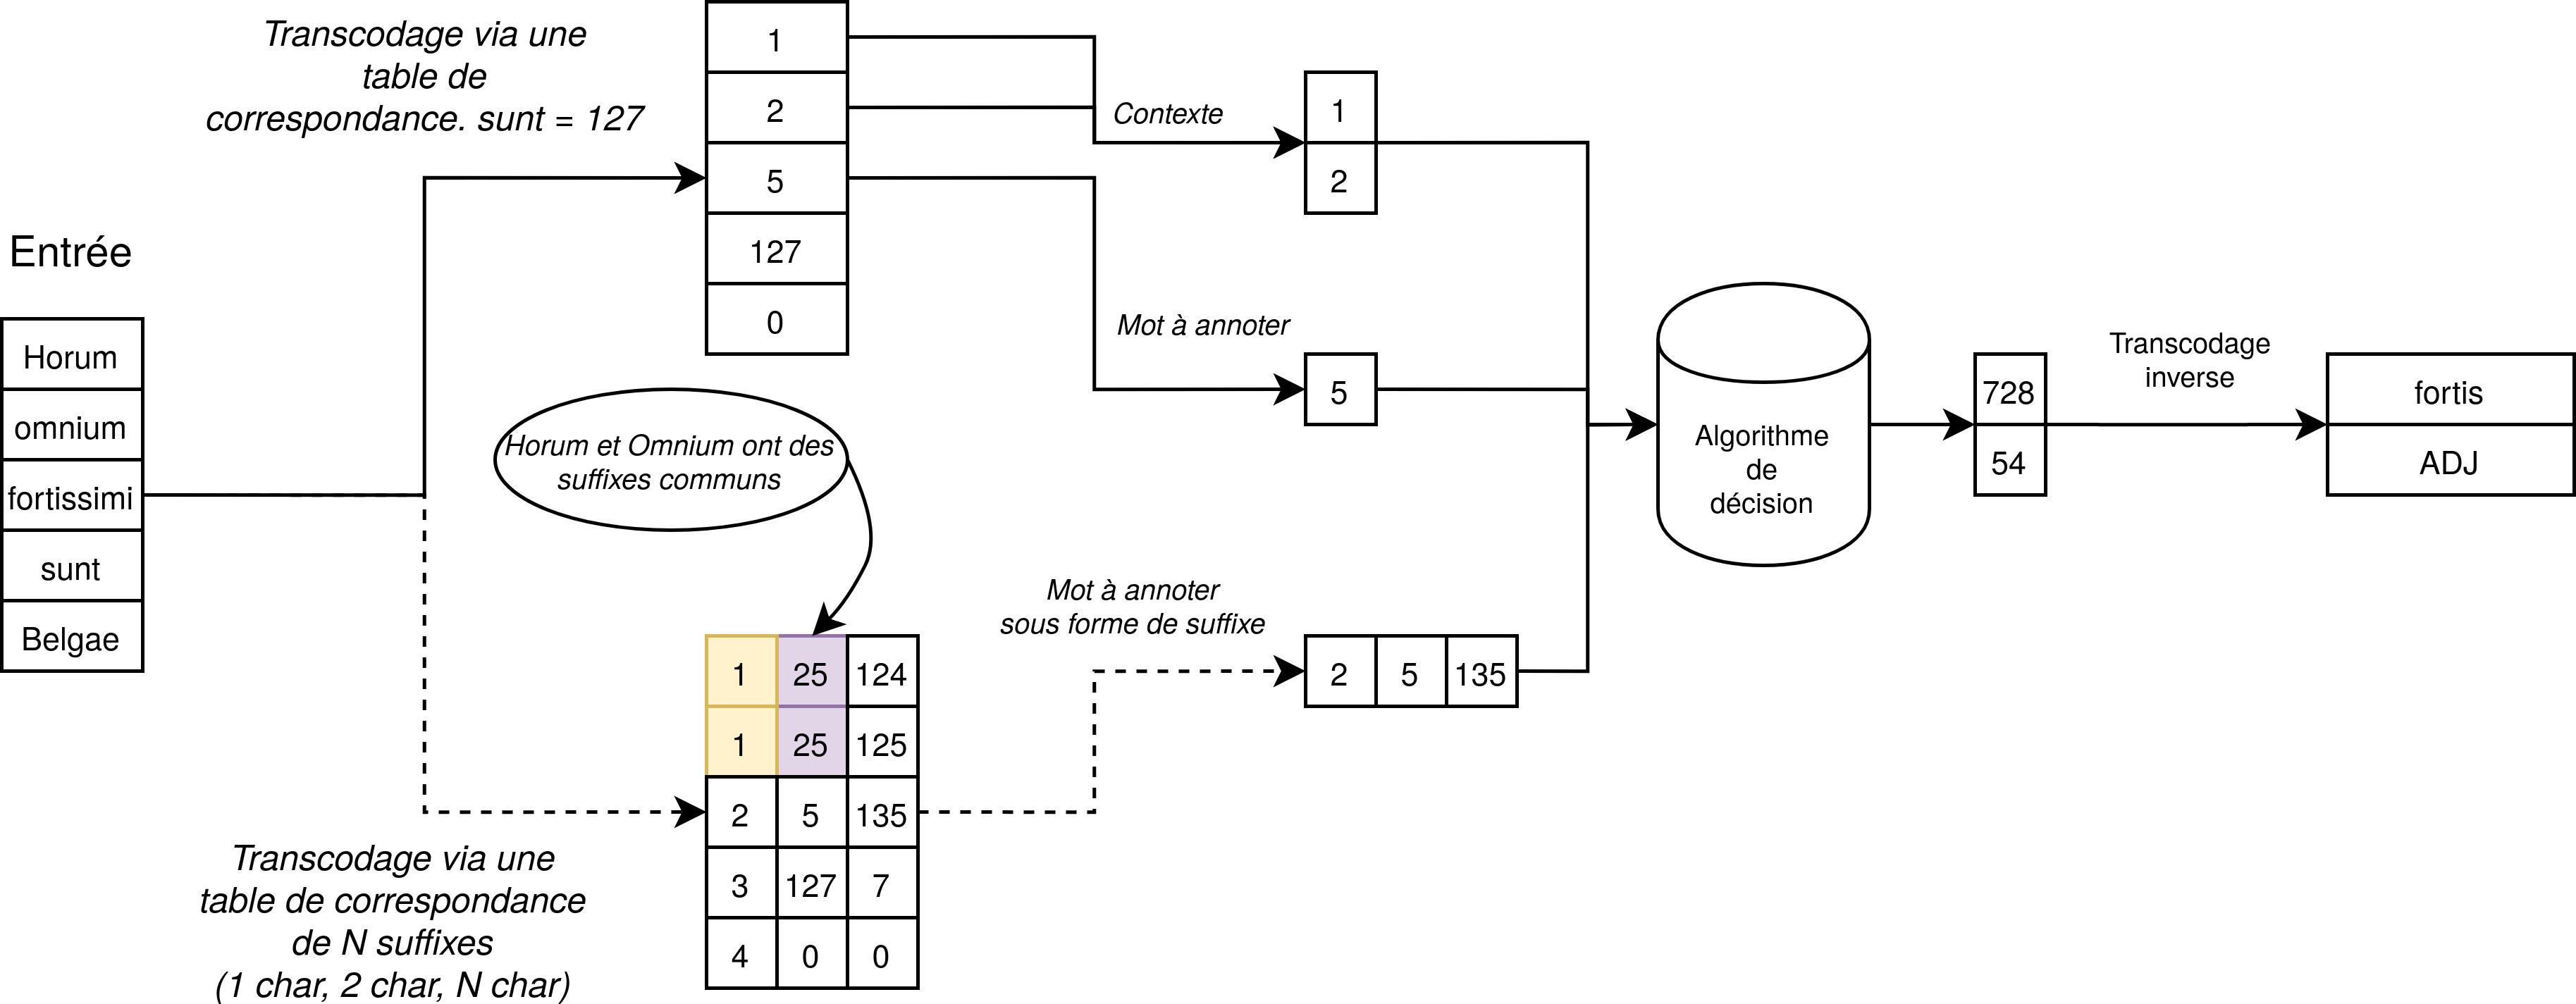
\includegraphics[width=\linewidth]{figures/chap3/outils/treetagger_type.png}
    \caption{Type de fonctionnement des outils de l'époque Treetagger. Une seule représentation des données est prise en compte au moment \enquote{d'un seul} calcul. Il s'agit principalement de modèles statistiques basés sur des probabilités d'apparition de phénomènes.}
    \label{lemmatisation:outils:type-treetagger}
\end{figure}

Le problème évident de ces lemmatiseurs reste aujourd'hui leur relation à un dictionnaire de forme et de lemmes qui ne leur permet pas (\textit{cf.} figure \ref{lemmatisation:outils:type-treetagger}), dans la majorité des cas, de prédire un lemme inconnu ou de gérer plus efficacement une forme inconnue en termes de lemmatisation. Les formes sont traitées telles quelles, ce qui pose, même s'ils prennent en compte des suffixes, rapidement des problèmes pour la lemmatisation ou l'annotation  de la POS dans le cadre du latin (avec des marques flexionnelles telles que \textit{-a} communes à la fois aux noms, aux participes, aux adjectifs, etc.).%exemple ? Vraiment difficile de savoir quoi dire ici...

\subsection{Les outils sur base de traduction (Milieu et fin des années 2010 et après)}

En 2016\footcite{kestemont_initial_2016}, Mike Kestemont propose une première version de Pandora\footcite{kestemont_lemmatization_2017}, un tagueur permettant à la fois la lemmatisation, l'annotation de la POS et des traits morphologiques en contexte. Sa particularité est de cibler le latin, à la fois médiéval et classique, en prenant en compte les difficultés inhérentes de cette langue: d'une part, une morphologie très lourde, beaucoup plus lourde que celle de l'anglais souvent pris comme cible par les développeurs de lemmatiseur; d'autre part, une syntaxe particulièrement libre. Ce travail se base alors sur l'état de l'art en traitement automatique des langues, à savoir des modèles d'apprentissage profond (\textit{deep learning}). Le modèle est constitué d'une couche d'\textit{embeddings}, d'un encodeur LSTM et de plusieurs décodeurs fonctionnant soit sur une base LSTM (pour le lemme), soit sur une couche linéaire (pour les tâches morpho-syntaxique).


\begin{figure}[h]
    \centering
    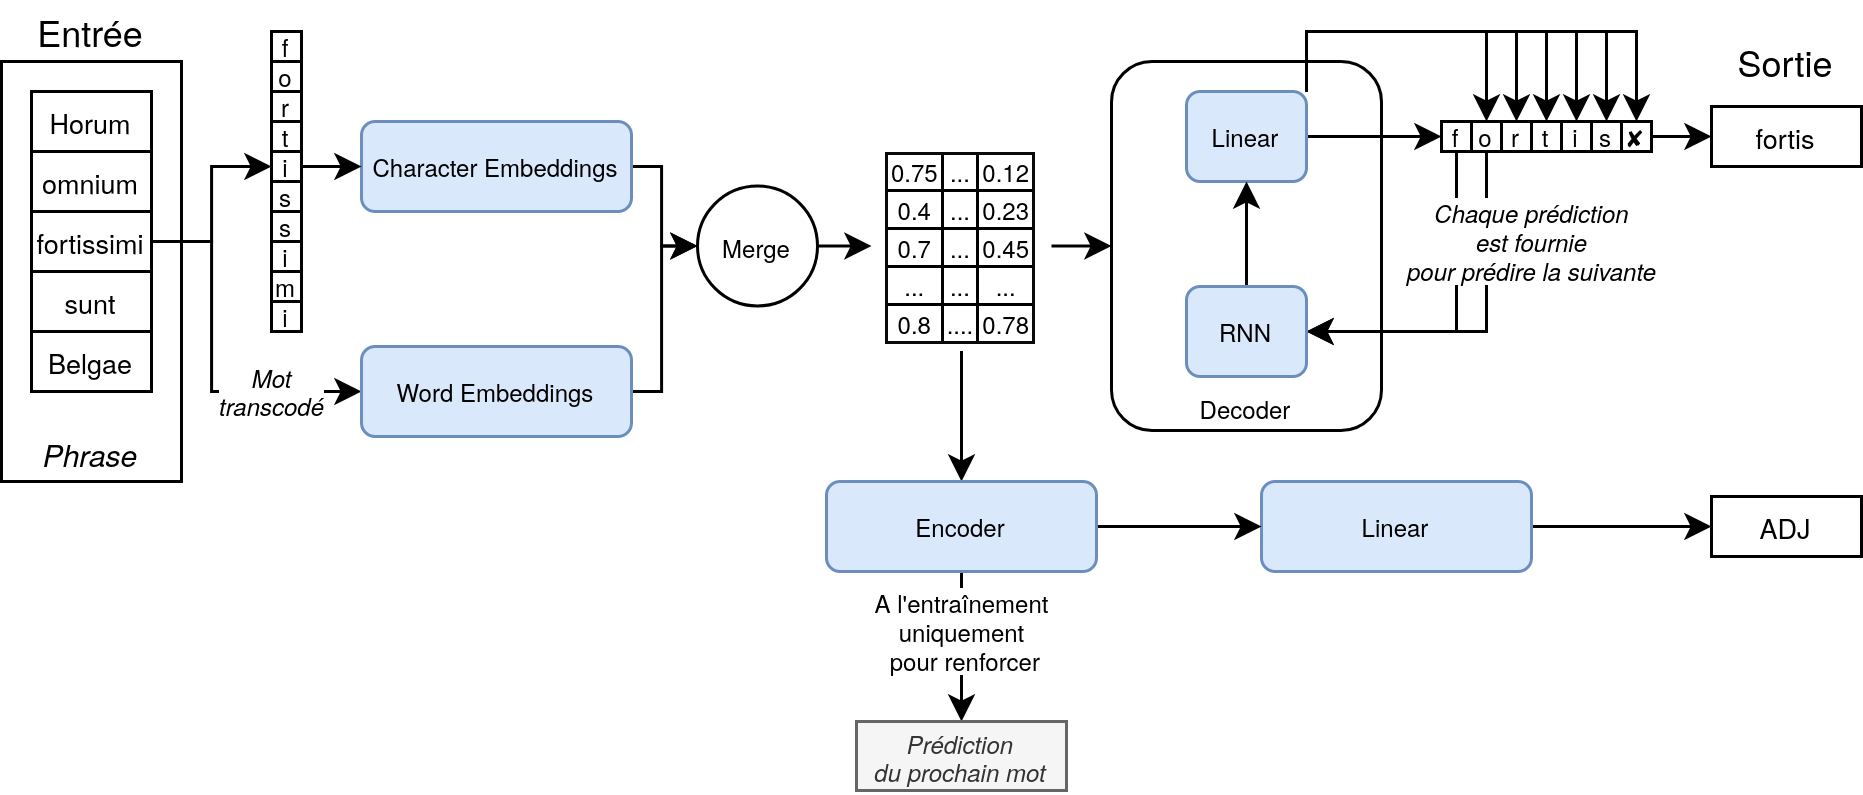
\includegraphics[width=\linewidth]{figures/chap3/outils/Pie.png}
    \caption{Représentation simplifiée de Pie. L'encodeur n'est utilisé que pour les classifications de mots et à l'entraînement comme support d'entraînement supplémentaire. Lettre par lettre, le lemmatiseur traduit la forme en un lemme. Bien que noté \textit{Embeddings}, le module de projection des caractères prend la forme au choix de CNN ou de RNN en plus d'une couche réelle d'\textit{Embeddings} classiques}
    \label{lemmatisation:outils:pie}
\end{figure}

Ce lemmatiseur est perfectionné par E. Manjavacas\footcite{manjavacas_improving_2019} qui propose une architecture de code plus souple permettant entre autres de tester plusieurs configurations. Il apporte des nouveautés telles qu'une meilleure gestion des caractères via des \textit{embeddings} en CNN (plus rapide) et la mise à disposition des modèles GRU pour les encodeurs et décodeurs. Le principe reste le même que pour la traduction automatique: quand pour ce dernier domaine on tente de traduire des mots en anglais à partir d'une phrase en français, \textit{pie} et les lemmatiseurs du même genre essayent de traduire chacune des lettres d'un \textit{token} en lettres de son lemme, une à une. De cette manière, il intègre des règles de lemmatisation telles que \textit{$\textrm{-ae} \rightarrow \textrm{-a}$}. Cela signifie aussi que ce lemmatiseur peut avoir tendance à créer des lemmes inexistants, tout en respectant une certaine forme de logique interne: potentiellement, les lemmes ne sont pas les bons, mais correspondent à ce que le lemmatiseur a estimé être une forme logique. % Faire une étude ici ?

\section{Corpus et méthodes d'évaluation}
\label{subsec:lemma_corpus}

\subsection{Les corpus disponibles}

Pour l'entraînement d'outils de lemmatisation, il existe très peu de corpus latins. On en compte quatre pour la période classique, utilisant deux dictionnaires de référence, mais trois référentiels de POS. Ces quatre corpus sont issus des projets Perseus, Proiel, Perseids et du LASLA. À l'exception de ce dernier, il sont tous à l'origine des corpus de treebank et non de lemmatisation: il semble qu'il n'y ait pas eu, historiquement, d'autres projets que ceux du LASLA pour la lemmatisation manuelle du latin classique.

Le corpus \textit{Perseus}\footnote{Aussi connu sous le nom de \textit{Latin Dependency Treebank}} est décrit dans son article programmatique de 2006\footcite{bamman_design_2006}. L'objectif de ce projet d'annotation ne concerne en aucun cas la lemmatisation: le terme \textit{lemma} n'est présent qu'une seule fois dans l'article initial pour près de 4000 mots et 10 pages de rédaction. Il est réalisé sous la direction de D. Bamman et G. Crane puis de G. Celano et de G. Crane. Dans les années précédant 2020, l'équipe de G. Crane s'est majoritairement focalisée sur le grec, qu'il s'agisse de l'expansion du corpus de textes édités ou de textes treebankés, résultant en une stagnation du corpus latin. D'ailleurs, ce corpus est le plus petit des corpus d'équipes (\textit{LASLA, Proiel, Perseus}): au mois d'avril 2020, celui-ci contenait 76~670 tokens, ponctuations et enclitiques compris, et ne comprenait aucune œuvre complète. Sa base de lemmes est dérivée du Lewis \& Short\footcite{shorts_latin_1958}, les POS ne sont pas éditées en contexte, mais la morphologie l'est.

Le corpus \textit{Harrington} est un corpus issu d'une pratique pédagogique de l'annotation du latin\footcite{noauthor_harrington_nodate} via la plate-forme \textit{Perseids}\footcite{almas_perseids_2016}. Il suit les mêmes recommandations en lemme et en morphologie que le corpus de \textit{Perseus}, mais diffère sur la grammaire de dépendance utilisée. Certaines œuvres de \textit{Perseus} sont réannotées avec cette grammaire, réduisant ainsi la taille cumulée des deux corpus. Contrairement au corpus \textit{Perseus}, il est encore en cours de production par les étudiants de D. Harrington. Au mois d'avril 2020, il contenait 120~029 tokens, enclitiques et signes de ponctuation compris et ne comprenait pas non plus d'œuvre complète. 

Le corpus \textit{PROIEL} est un corpus de projet plurilingue d'étude du \textit{Nouveau Testament} dans les langues indo-européennes anciennes\footcite{haug_creating_2008}. Il suit les mêmes recommandations en morphologie et en lemmatisation que les projets \textit{Perseus} et \textit{Harrington} mais diffère sur ses annotations de POS et sur la grammaire de dépendance utilisée. Corpus toujours en activité, il ne comprend aucune œuvre complète, mais est assurément le corpus le plus important des trois issus du Lewis \& Short. Contrairement aux deux précédents, c'est une collection qui, comme le LASLA, est d'abord un projet fondé par des linguistes et grammairiens avant d'être un produit de chercheurs en littératures ou d'enseignants comme G. Crane et D. Harrington\footnote{Nous parlons ici de fondation, G. Celano étant lui aussi un linguiste.}.

\begin{table}[h]
\centering
\resizebox{\textwidth}{!}{%
\begin{tabular}{l|rrrrrr}
\toprule
        & Tokens             & Ponctuation & Nombre     & Nombre  & Lemmes & Dictionnaire \\ 
        &                    &   comprise  &  d'auteurs &  de textes & uniqes & \\   \midrule
PROIEL  & 225~064            & Non                  & 5                & 6  & 7~246              & Lewis\footnotemark\\
Perseus & 79~670             & Oui                  & 12               & 12 & 6~017              & Lewis \\
Harrington & 120~029             & Oui                  & 9               & 12 &  7~675             & Lewis\\
LASLA   & \textbf{1~630~825} & Non                  & \textbf{18}                 &  \textbf{100+}     & 25~135          & Forcellini \\ \bottomrule
\end{tabular}%
}
\caption{Résumé des informations sur les quatre corpus disponibles. Il existe 137 œuvres au sens du LASLA, mais certaines sont des des découpes inhabituelles, nous préférons donc la notation 100+ ici.}
\label{tab:lemmatisation:corpus-entrainement}
\end{table}
\footnotetext{Légèrement modifié.}

Le corpus du LASLA, qui sera retenu de par sa taille et de par sa diversité, est un corpus dont nous avons précédemment parlé et dont la constitution a commencé dans les années 1960\footcites{delatte_laboratoire_1961}{BodsonCodification1966}. Contrairement aux autres, il ne possède aucun texte à partir du II\textsuperscript{e} siècle de notre ère, ce qui en fait sa plus grande faiblesse. L'apprentissage machine reposant principalement sur le nombre de données et leur variété, il n'était pas envisageable d'utiliser une autre source que celle produite par les philologues belges. Par ailleurs, des essais en début de thèse nous avaient prouvé l'incapacité des modèles à prédire des résultats très fiables à partir des données de \textit{Perseus} ou de \textit{Proiel}: à cause de la taille beaucoup trop faible de \textit{Perseus}, le modèle ne s'entraînait pas assez, tandis qu'à cause des données peu variées de \textit{PROIEL}, il ne connaissait que la \textit{Vulgate} et quelques mots de Cicéron.

\begin{figure}
    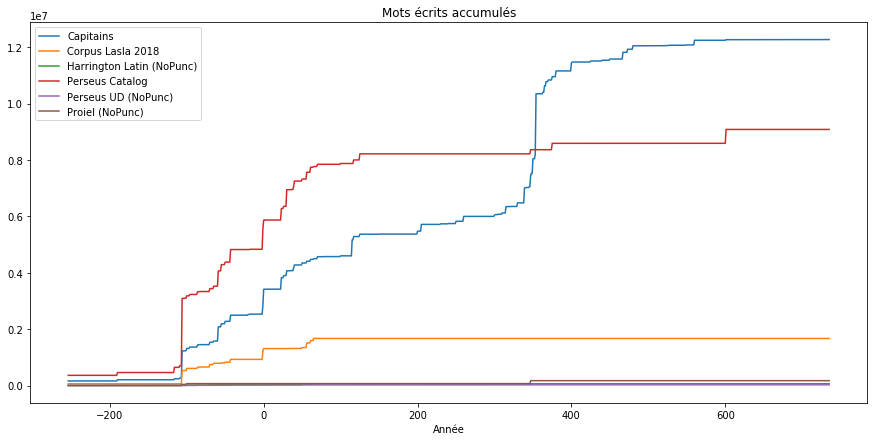
\includegraphics[width=\linewidth]{figures/chap3/corpus/tokens_per_year.png}
    \caption{Tokens accumulés, par année, en fonction des corpus latins bruts accessibles en \textit{open access} (\textit{Capitains}) ou du nombre estimé  par le \textit{Perseus Catalog}.}
    \label{fig:lemmatisation:corpus-entrainement}
\end{figure}

\subsection{Le corpus du LASLA: choix d'étiquetage}

Le corpus du LASLA utilisé présente 1~630~825 tokens dans la version à laquelle nous avons accès. Il est constitué de 25~135 lemmes, 1~008 types d'annotations morphologiques (\textit{par exemple}  \texttt{Ablatif Pluriel} et \texttt{Deuxième personne Pluriel Indicatif Parfait Actif}) pour 28 grandes catégories syntaxiques (nom, verbe, préposition, etc.) divisées là où il est possible de le faire en déclinaisons (nom1, nom2, etc.). On trouve dans le corpus de très rares erreurs d'annotation, principalement due à une information partielle, et celles-ci semblent marginales au regard du nombre de \textit{tokens}. Le LASLA a fait le choix d'un étiquetage pour majeure partie morphosyntaxique avec désambiguïsation en contexte, laissant quelques cas d'ambiguïtés quand le doute était suffisamment fort pour que l'annotateur ou l'annotatrice ne fasse pas choix. Nous revenons donc sur deux choix affectant les résultats d'analyse automatique: d'une part l'annotation du genre, d'autre part l'annotation des verbes à formes composées.

\subsubsection{Le cas du genre}

Le LASLA a fait le choix de réserver \enquote{l'indication du genre pour les adjectifs, numéraux, les adjectifs-pronoms, les formes déclinées du verbe, hormis le gérondif}\footcite[p.~27]{BodsonCodification1966} dont la répartition est décrite en table \ref{table:lasla:genders-par-pos}. Ce choix a pour conséquence de laisser le genre des noms inconnus: on ne pourra distinguer, dans le contexte de notre recherche, les noms par leur genre masculin, neutre ou féminin, l'information faisant défaut. On pourrait imaginer un travail de réannotation de tous les lemmes dont la POS est NOM avec leur genre quand il est fixe. Ce travail serait potentiellement riche d'influence sur les statistiques finales. Par ailleurs, le genre, à l'inverse du cas et du nombre, n'a pas été analysé en contexte (c'est-à-dire syntaxiquement), mais hors contexte (c'est-à-dire morphologiquement), ce qui laisse des ambiguïtés comme \textit{bonum} qui est à la fois masculin et neutre à l'accusatif singulier. Dans ce contexte, le LASLA crée trois genres morphologiques additionnels aux genres classiques: le Commun, le Masculin-Féminin et le Masculin-Neutre (dont la répartition dans le corpus d'entraînement est visible en \ref{table:lasla:genders-par-corpus}). L'explication derrière ce choix, disponible dans l'article de Bodson\footcite{BodsonCodification1966}, réside dans un problème technique de 1966, qui risquait de poser un problème d'export. Malheureusement, ce choix, aujourd'hui pourtant possible à résoudre, crée une forme de dette technique pour plus de 300 000 mots. On remarque cependant, à la marge, par alignement avec les formes possibles sur \textit{Collatinus} \footnote{\textit{Cf.} annexes numériques.} qu'une analyse en contexte a été probablement faite à la marge (\textit{cf.} table \ref{table:lasla:genders-alignement}).

\begin{table}[!htb]
    \begin{minipage}[t]{.4\linewidth}
        \centering
        \resizebox{\textwidth}{!}{%
            \begin{tabular}{l|rrr}
            \toprule
                     & PRO    & VER    & ADJ    \\ \midrule
            Com      & 30 004 & 14 841 & 26 384 \\
            Fem      & 37 177 & 16 393 & 34 292 \\
            Masc     & 42 598 & 18 785 & 24 331 \\
            MascFem  & 8 398  & 3 968  & 17 477 \\
            MascNeut & 25 459 & 12 170 & 30 815 \\
            Neut     & 46 479 & 11 151 & 25 381 \\ \bottomrule
            \end{tabular}
        }
        \caption{Répartition des genres par POS}
        \label{table:lasla:genders-par-pos}
    \end{minipage}% \quad
    \hspace{0.19\linewidth} 
    \begin{minipage}[t]{.4\linewidth}
        \centering
        \resizebox{\textwidth}{!}{%
            \begin{tabular}{l|rrr}
            \toprule
                       & Train   & Dev   & Test   \\ \midrule
            Fem        & 77 907   & 986   & 8 971   \\
            Masc       & 76 213   & 925   & 8 576   \\
            Neut       & 73 899   & 993   & 8 119   \\
            Com        & 63 304   & 789   & 7 136   \\
            MascFem    & 26 492   & 322   & 3 030   \\
            MascNeut   & 61 031   & 743   & 6 671   \\
            N/A        & 1 153 885 & 14 788 & 130 465 \\
            \textit{- Dont noms} & 433 117  & 5 634  & 48 840  \\ \bottomrule
            \end{tabular}
        }
        \caption{Répartition des genres par corpus}
        \label{table:lasla:genders-par-corpus}
    \end{minipage} 
\end{table}


\begin{table}[h]
\centering
\begin{tabular}{l|lll}
\toprule
         & MascNeut & MascFem & Com    \\ \midrule
0        & 783      & 653     & 1 478  \\
1        & 219      & 3 863   & 33     \\
2        & \textbf{65 852}   & \textbf{25 155}  & 2 512  \\
3        & 1 591    & 172     & \textbf{67 206} \\ \bottomrule
\end{tabular}
\caption{Nombre de genres possibles par alignement Forme+Cas+Nombre via \textit{PyCollatinus}\footcite[\textit{PyCollatinus} est une traduction en python de \textit{Collatinus, cf. }]{thibault_clerice_2018_1243076}. Les informations qui ne sont pas en gras montrent une différence possible entre une annotation morphologique et morphosyntaxique. Il peut aussi s'agir d'erreurs de \textit{PyCollatinus}.}
\label{table:lasla:genders-alignement}
\end{table}

\subsubsection{Les formes verbales composées et leur annotation}

Un autre choix du LASLA a été d'annoter les participes avec le temps de la forme composée: pour \textit{amatus sum}, \textit{amatus} portera l'information du temps (\texttt{parfait}), du mode (\texttt{indicatif}), de la personne (\texttt{1}) et du genre (\texttt{Masc}) sans porter l'information du cas pourtant présent morphologiquement. Au contraire, \textit{sum} portera la simple annotation de verbe auxiliaire. Cela pose un problème de confusion pour une même forme \textit{amatus} qui peut être annotée comme simple participe parfait passif avec une annotation \texttt{Mode Voix Temps} ajoutée à une annotation \texttt{Genre Nombre Cas}, et une forme amatus (ellipse ou présence de) sum qui elle sera annotée aussi avec \texttt{Mode Voix Temps}, mais sans le triplet \texttt{Genre Nombre Personne}. Dans cette optique, \textit{amatus} peut représenter 6 formes conjuguées hors participes, 7 pour le neutre \textit{amatum} (\textit{cf.} Table \ref{table:amatus_forms}). %
%
% Exemple pour le parfait passif
%
Ainsi, dans la phrase du \textit{De Amicitia} de Cicéron, \enquote{\textbf{uidetis} in tabella iam ante quanta \textbf{facta} labes primo Gabinia lege biennio post Cassia }, \textit{uidetis} est annoté à la 2\textsuperscript{e} personne du pluriel indicatif présent actif là où \textit{facta} est annoté à la 3\textsuperscript{e} du singulier subjonctif parfait passif. Si cette approche est particulièrement intéressante dans un contexte d'analyse morphosyntaxique, elle est d'autant plus difficile à différencier d'un \textit{facta} nominatif pour un lemmatiseur automatique. Quelle différence en effet peut être faite dans la phrase \enquote{non oculi tacuere tui \textbf{conscriptaque} uino mensa nec in digitis littera nulla fuit} (Ovid. Her. 2.5.17 sqq.) avec le cas précédent ? % D'ailleurs, n'est-ce pas un raté ??

% Fin d'exemple

\newpara

\begin{table}[h]
\centering
\begin{tabular}{@{}lll@{}}
\toprule
Forme & Mode & Temps \\ \midrule
amatus (sum) & Indicatif & Parfait \\
amatus (eram) & Indicatif & Plus-que-parfait \\
amatus (ero) & Indicatif & Futur antérieur \\
amatus (sim) & Subjonctif & Parfait \\
amatus (essem) & Subjonctif & Plus-que-parfait \\
amatus (esse) & Infinitif & Parfait \\
amatum (iri) & Infinitif & Futur \\ \bottomrule
\end{tabular}
\caption{Annotations possibles pour la forme \textit{amatus} dans le LASLA, hors participes}
\label{table:amatus_forms}
\end{table}

Cette multiplicité d'annotation peut rendre difficile le travail de l'annotation automatique, car elle sous-entend une capacité pour le lemmatiseur de reconnaître les formes au nominatif utilisées de manière adjectivale des formes utilisées comme verbe principal ou verbe subordonné. Nous proposons en \ref{subsec:training:lasla-modification} une analyse de modifications pour une simplification du travail du modèle, en vue de la création d'un modèle morphologique et non morphosyntaxique plus performant.

\subsubsection{Création de lemmes, lexicographie, lexicalisation}

La question de la lexicalisation dans le cadre de la lemmatisation est particulièrement importante, en ce qu'elle peut définir ce qui fait lemme. Doit-on pour autant confondre lexicalisation, création de lemme et création lexicographique ? Au sens original du terme \textit{lemme}, la création lexicographique et celles d'un lemme sont confondues, mais le glissement du dictionnaire vers la base de référentiel permet aussi de distinguer les deux et de faire des choix. Par exemple, dans les données du LASLA, on trouvera les lemmes \textsc{Romani}, les Romains, et \textsc{romanus}, romain en adjectif, quoique le \textit{Forcellini}, dictionnaire source utilisé par le LASLA, ne donne que \textsc{Romanus}, et uniquement dans son \textit{Onomasticon}. Cette distinction se retrouve par ailleurs pour l'ensemble des noms de peuples ou d'habitants. Ce résultat est celui du choix de la primauté de la POS comme séparateur des lemmes: à partir du moment où les formes dans le LASLA sont annotées en fonction d'un couple Lemme-POS intangible, la substantivation d'un adjectif donne lieu à la création d'un lemme et donc d'une nouvelle entrée. L'alternative rejetée est celle d'une annotation de la POS en contexte, quelque soit la POS traditionnelle du lemme: on pourrait ainsi avoir un participe passé substantivé en POS NOMcom, mais avec les traits morphologiques du verbe. Ce choix du LASLA n'est pas évident et peut impliquer, dès lors qu'il y a lexicalisation d'adjectifs substantivés, même dans un cas unique ou du moins réduit, une création de lemmes. De fait, doit-on prendre la lexicalisation, c'est-à-dire d'une certaine manière la prise d'autonomie d'une forme pour un nouvel usage, comme phénomène initiateur de création de lemme ? Cette question est difficile, et le débat peut être complexe. Le défi de la diachronie se pose avec l'annotation, à partir du même référentiel, de faire des choix certains et solides. Cela reste un choix et il est clair que chacune des méthodes a ses avantages, et qu'il reste important de quantifier leur impact en termes de créations d'entrées\footnote{Dans le dictionnaire du LASLA, 12,77\% des lemmes adjectifs peuvent correspondre à des participes et des adjectifs, 12,67\% des adverbes correspondent à des ablatifs de NOMcom, 42,96\% des adverbes correspondent à des instrumentaux en -e ou des formes en -iter d'adjectifs et enfin 23,87\% des lemmes de noms communs peuvent correspondre à des adjectifs substantivés.}.

Il ne s'agit pas pour autant de la seule option visant à limiter le nombre de lemmes ou du moins la possibilité de devoir créer des lemmes à occurrence unique. Parmi les autres choix d'annotation, on peut imaginer, dans le cadre où les adverbes dérivés d'adjectifs ou de noms sont des survivances d'un cas instrumental en \textit{-e} long, d'un ablatif singulier pour les substantifs, de ne pas créer de lemme, mais d'annoter, en quasi-uchronie, sur le lemme supposé d'origine ? Serait-il intéressant dans cette situation de répertorier les termes ici sous un cas perdu, étymologique, quand cela est nécessaire, et d'annoter la POS en contexte ? Si ce choix ne semble par exemple pas si facile dans le cas des adjectifs, les substantifs à l'ablatif grammaticalisés du type \textsc{nocte} laissent une part d'interprétation assez forte, la grammaticalisation n'étant pas toujours facilement identifiable\footcite{fruyt_adverbes_2008}, en dehors des cas particuliers de comparatifs qui ne sauraient bien sûr être appliqués à un nom (comme un \textit{noctissime}%\begin{comment}\footnote{Si l'on revient d'ailleurs à \cite{meillet_levolution_1922}, s'agit-il d'une grammaticalisation qui donne lieu à une nouvelle déclinaison au niveau du degré ou une création par analogie dans ce cas précis ?}\end{comment}
ou bien \textit{magis merito} relevé par Claude Brunet\footcite{brunet_merito_2008}). Le risque de cette méthode est clair: dans une volonté d'annotation presque reconstructionniste, on risque de rendre ce travail, lorsqu'il est manuel, encore plus difficile. Dans les différents degrés de création lexicale, il faut donc différencier les problèmes de reconstruction morphologiques (adjectif adverbialisé ou nom adverbialisé à l'instrumental), les problèmes dus à une POS figée par le lemme à la place d'une annotation en contexte (\textsc{romanus} et \textsc{Romani}). Il existe bien sûr des solutions partielles permettant de conserver les données dans l'état, à savoir de créer une base de connaissances claire connectant ensemble ces prises d'autonomie. C'est entre autres une des missions que s'est attribuées le projet de l'ERC LiLa qui court jusqu'en 2023\footcite{passarotti_interlinking_2020} et pour lequel - par exemple - existe une entrée \textit{merito}. Cependant, au moment de la rédaction, le seul type de relation identifié est celle de \textsc{merito} avec une base de lemme (au sens de dérivation) \textsc{mereo}, bien qu'une relation - peut-être trop faible - \textit{isHypoLemma} existe et relie par exemple \textsc{meritus} et \textsc{mereo/mereor}.

\section{Configurations évaluées et processus décisionnel}

\subsection{Impact du choix d'étiquetage des formes passives ou déponentes composées}
\label{subsec:training:lasla-modification}

Le choix d'annoter des formes simples (les participes) par le temps de la forme composée provoque une difficulté d'apprentissage importante. En retirant du lot les formes adjectivales, le \textit{micro-average} des formes simples est de 97,67 là où la même mesure pour les formes composées stagne à 73,30. Par ailleurs, le \textit{macro-average} et l'\textit{écart-type} montre ces disparités (\textit{cf.} Table \ref{table:lasla:formes-simples-formes-composees})\footnote{Le \textit{micro-average} s'intéresse à la moyenne sur l'ensemble des formes tandis que le \textit{macro-average} se concentre sur la moyenne des scores par catégories.}. La déviation standard des temps simples peut-être majoritairement expliquée par des formes extrêmement rares ou erronées comme l'impératif présent passif (1 occurrence sur le corpus de test, 0 de précision) ce qui appuie l'importance des deux mesures de \textit{micro-} et de \textit{macro-average}. Pour gérer ce problème, on propose de traduire les annotations automatiquement pour ces parfaits: les temps composés utilisant le parfait passif passent en \textsc{Mode-Temps-Voix} à \textsc{Par-Pft-Voix} (où voix correspondra donc à passif, déponent ou semi-déponent). Les modes composés de l'infinitif sont annotés avec le cas, il est donc conservé. Les autres modes passent automatiquement au nominatif et perdent l'annotation de personne. Cette conversion double le nombre de participes futurs, augmente de moitié le nombre de participes parfaits passifs et n'a bien sûr aucune incidence sur les participes présents (\textit{cf.} Table \ref{table:lasla:correction-temps}.) Les résultats (Table \ref{table:lasla:formes-simples-formes-composees}) sont sans appel: l'intégralité des annotations de formes composées (qui correspondent désormais aux participes) connaît un bond de 40 points en \textit{macro-average} et 18 points en \textit{micro-average}. L'écart-type reste fort dans la mesure où certaines classes sont trop rares ou fautives (par exemple, les éléments annotés syntaxiquement comme des participes futurs passifs sont dans leur intégralité des participes parfaits passifs et n'ont pas été touchés par cette modification.). Les classes fautives restantes posent un problème, mais leur poids dans l'entraînement est assez négligeable pour ne pas influer la reconnaissance des participes parfaits passifs, participes futurs actifs et participes présents actifs (Table \ref{table:lasla:main-particips}).

% ToDo: L'annotation de l'auxiliaire ?

\begin{table}[h]
\centering
\begin{tabular}{@{}l|r|lll|lll@{}}
\toprule
                                &         & \multicolumn{3}{l}{Pré-correction} & \multicolumn{3}{l}{Post-correction} \\ \midrule
Précision                       & Support      & Macro    & Écart-Type   & Micro    & Macro     & Écart-Type   & Micro    \\ \midrule
Verbes (hors N/A)               & 39~465        & 65,24   & 39,92        & 93,36    & 90,61     & 22,33        & 96,67   \\
Formes simples                  & 31~254        & 94,17   & 16,79        & 97,80    & 94,17     & 16,77        & 97,86   \\
Formes Composées                & 7~027         & 35,70   & 35,66        & 73,78    & 76,36     & 38,10        & 91,74   \\
- \textit{dont participe}       & 4~946         & 64,30   & 36,10        & 80,87    & 76,36     & 38,10        & 91,74   \\
Formes “adjectivales”           & 1~173         & 90,67   & 15,39        & 92,27    & 93,78     & 05,95        & 94,33   \\ \bottomrule
\end{tabular}
\caption{Précision en fonction des catégories de temps sur la base forme composée/simple et les scores de la table \ref{table:lasla:verb-scores}. Les formes autres correspondent au supin, au gérondif, et à l'adjectif verbal, les formes composées contiennent la catégorie participe.}
\label{table:lasla:formes-simples-formes-composees}
\end{table}

% Check participe futur passif ?

\begin{table}[h]
\centering
\begin{tabular}{l|rrr|rrr}
\toprule
 & \multicolumn{3}{c}{Pré-correction} & \multicolumn{3}{c}{Post-correction} \\ 
 & Test & Dev & Train & Test & Dev & Train \\ \midrule
Par-Fut-Act & 214 & 20 & 1726 & 445 & 46 & 3908 \\
Par-Fut-Dep & 14 & 1 & 121 & 30 & 2 & 209 \\
Par-Fut-Pass & 0 & 0 & 0 & 3 & 0 & 54 \\
Par-Fut-SemDep & 1 & 0 & 13 & 3 & 1 & 28 \\
Par-Perf-Act & 1 & 0 & 2 & 1 & 0 & 2 \\
Par-Perf-Dep & 363 & 32 & 3267 & 653 & 65 & 6203 \\
Par-Perf-Pass & 2927 & 309 & 25334 & 4391 & 526 & 38030 \\
Par-Perf-SemDep & 23 & 5 & 217 & 58 & 11 & 537 \\
Par-Pres-Act & 1210 & 137 & 10935 & 1210 & 137 & 10935 \\
Par-Pres-Dep & 188 & 20 & 1493 & 188 & 20 & 1493 \\
Par-Pres-Pass & 0 & 0 & 1 & 0 & 0 & 1 \\
Par-Pres-SemDep & 5 & 5 & 70 & 5 & 5 & 70 \\ \bottomrule
\end{tabular}
\caption{Résultats sur le décompte de participes des conversions automatiques temps composés vers participe. On remarque a posteriori au moins 2 lignes problématiques (Par-Perf-Act) et (Par-Pres-Pass). Le poids de cette erreur sur un macro-average sera important, mais négligeable sur le micro-average}
\label{table:lasla:correction-temps}
\end{table}

\begin{table}[ht]
\centering
\resizebox{\textwidth}{!}{%
\begin{tabular}{l|rrrr|rrrr}
\toprule
 & \multicolumn{4}{c}{Pré-correction}     & \multicolumn{4}{c}{Post-correction} \\ \midrule
              & Précision & Rappel        & F1-Score & Support & Précision     & Rappel        & F1-Score      & Support \\ \midrule
Par-Fut-Act   &   91      &   89          & 90       & 214     & \textbf{97}   & \textbf{99}   & \textbf{98}   & 445     \\
Par-Perf-Pass &   76      &   83          & 79       & 2927    & \textbf{91}   & \textbf{94}   & \textbf{93}   & 4391    \\
Par-Pres-Act  &   94      & \textbf{98}   & 96       & 1210    & \textbf{95}   & 96            & 96            & 1210    \\ \bottomrule
\end{tabular}{}%
}
\caption{Résultats sur les trois formes principales du participe. En dehors d'un avantage de 2 points sur le rappel des participes présents actifs, tous les autres scores connaissent une augmentation notable, malgré une augmentation nette du nombre de données à tester.}
\label{table:lasla:main-particips}
\end{table} 

\subsection{Méthode(s) d'entraînement et résultats préliminaires}

L'entraînement du lemmatiseur Pie nécessite deux choses: il lui faut d'une part un corpus divisé en trois (d'entraînement, d'évaluation et de test), d'autre part, une série d'hyperparamètres concernant l'architecture du modèle et sa méthode d'apprentissage. Les deux ne sont pas indépendants: un corpus extrêmement riche d'une langue à forte variation morphologique ou orthographique demande \textit{a priori} un réseau plus complexe. Dans un premier temps, nous reviendrons sur l'importance de la connaissance du corpus d'entraînement et des potentielles adaptations qu'il faut faire à la marge. Ensuite, nous parlerons des différentes stratégies appliquées pour obtenir le meilleur modèle et proposerons un retour sur ces méthodes.

\subsubsection{Particularités du corpus et prétraitement}

Le corpus du LASLA présente de nombreuses particularités, propres à son statut de corpus annoté manuellement en vue de l'étude de la langue. C'est un corpus que l'on pourrait qualifier d'éditorialisé: des choix de présentation forts sont faits. Parmi ces choix, 
\begin{itemize}
    \item Le corpus ne présente aucune ponctuation syntaxique (coupure de phrase, marque de dialogue): les seuls signes de ponctuation sont réservés aux abréviations. Les phrases sont manuellement coupées au moment de l'annotation par les éditeurs de données. 
    \item Il utilise des parenthèses et des chevrons pour traiter les formes composées du type \textit{scripti <sunt>} et son inverse \textit{<scripti> sunt}.
    \item Il contient des apostrophes marquant des élisions  telles que \textit{venu'}, et des points pour les abréviations telles que \textit{Tib.}. Plus rarement et uniquement pour les fragments, les points indiquent des manques.
    \item Il n'utilise normalement pas de v minuscule ou de j. Leur présence extrêmement rare étant réservée à des oublis de correction. À l'inverse, on ne trouve pas de U majuscule.
    \item Les majuscules ne sont présentes que pour les noms propres et les adjectifs identifiant des peuples. Aucune majuscule n'est présente pour identifier des débuts de phrases.
    \item Le grec est translittéré en betacode, entouré d'un \$ de chaque côté: \enquote{\textit{Graeci \$pa/qh\$ nominant}} pour \textit{πάθη}.
    \item Certains couples de tokens sont considérés comme relevant d'un seul lemme: \textsc{usu capio}, \textsc{usu verio}, \textsc{res publica}, \textsc{bene dico}, \textsc{bene facio}, etc.
    \item Les lemmes sont désambiguïsés via des indicatifs numériques (de 1 à 5) ou des lettres (A, N) (pour les noms propres ou les peuples).
    \item Les lemmes sont en toute majuscule.
    \item Les nombres romains sont lemmatisés en toutes lettres et ne sont pas normalisés: on trouve ainsi \textit{XIIII} lemmatisé en \textsc{QUATVORDECIM}.
\end{itemize}
Ces particularités demandent un prétraitement important qui a pu varier en fonction des résultats. Pour anticiper ces problèmes, nous avons développé le programme Protogénie qui permet de prétraiter un corpus et surtout de garder en mémoire les éléments composant les corpus \textit{train}, \textit{dev} et \textit{test}. Nous proposons donc une chaîne de prétraitement permettant de normaliser les points d'entrée, y compris pour \enquote{simplifier} la tâche d'apprentissage du lemmatiseur. Ainsi, on présente les lemmes en minuscules, sauf pour les noms propres qui conservent une majuscule à l'initiale. Les nombres romains sont traduits en nombres arabes et les lemmes simplifiés en leur équivalent: \textit{XIIII} et son lemme \textsc{QUATVORDECIM} deviennent tous les deux 14. Sur ce point, l'effort de traduction ne relève pas des mêmes mécaniques que pour les autres lemmes: les règles flexionnelles ne sauraient être comparées aux règles de formation mathématique des formes. Or, pour éviter un apprentissage 1 à 1 (forme pour lemme) ou éviter un bruit introduit dans la compréhension du modèle flexionnel, on préfère traiter ces formes différemment, au choix en prétraitant l'information (à force de reconnaissance par règles des nombres romains) ou en conservant comme lemme la forme (\textit{XIII} lemmatisé \textsc{XIIII}). Dans un premier temps, on essaie sur ce point une configuration qui remplace les nombres supérieurs à 3 par 3, conservant ainsi les nombres 1, 2 et 3 et réduisant la taille des \textit{embeddings}. Par ailleurs, ce même outil sert à séparer la morphologie en autant de colonnes nécessaires. Une fois les corpus produits, on applique 3 fonctionnalités supplémentaires: la correction des temps composés (cf. \textit{supra} \ref{subsec:training:lasla-modification}), le recollage des clitiques aux termes qui les précèdent et leur identification dans le lemme afin de faire reposer la responsabilité de cette tâche au lemmatiseur, et enfin, l'ajout aléatoire de majuscules en début de phrases et à certains mots de manière aléatoire afin de déjouer un surapprentissage liant majuscule à l'initiale et noms propres.

\subsubsection{Besoin d'optimisation}

\begin{figure}[ht]
    \centering
    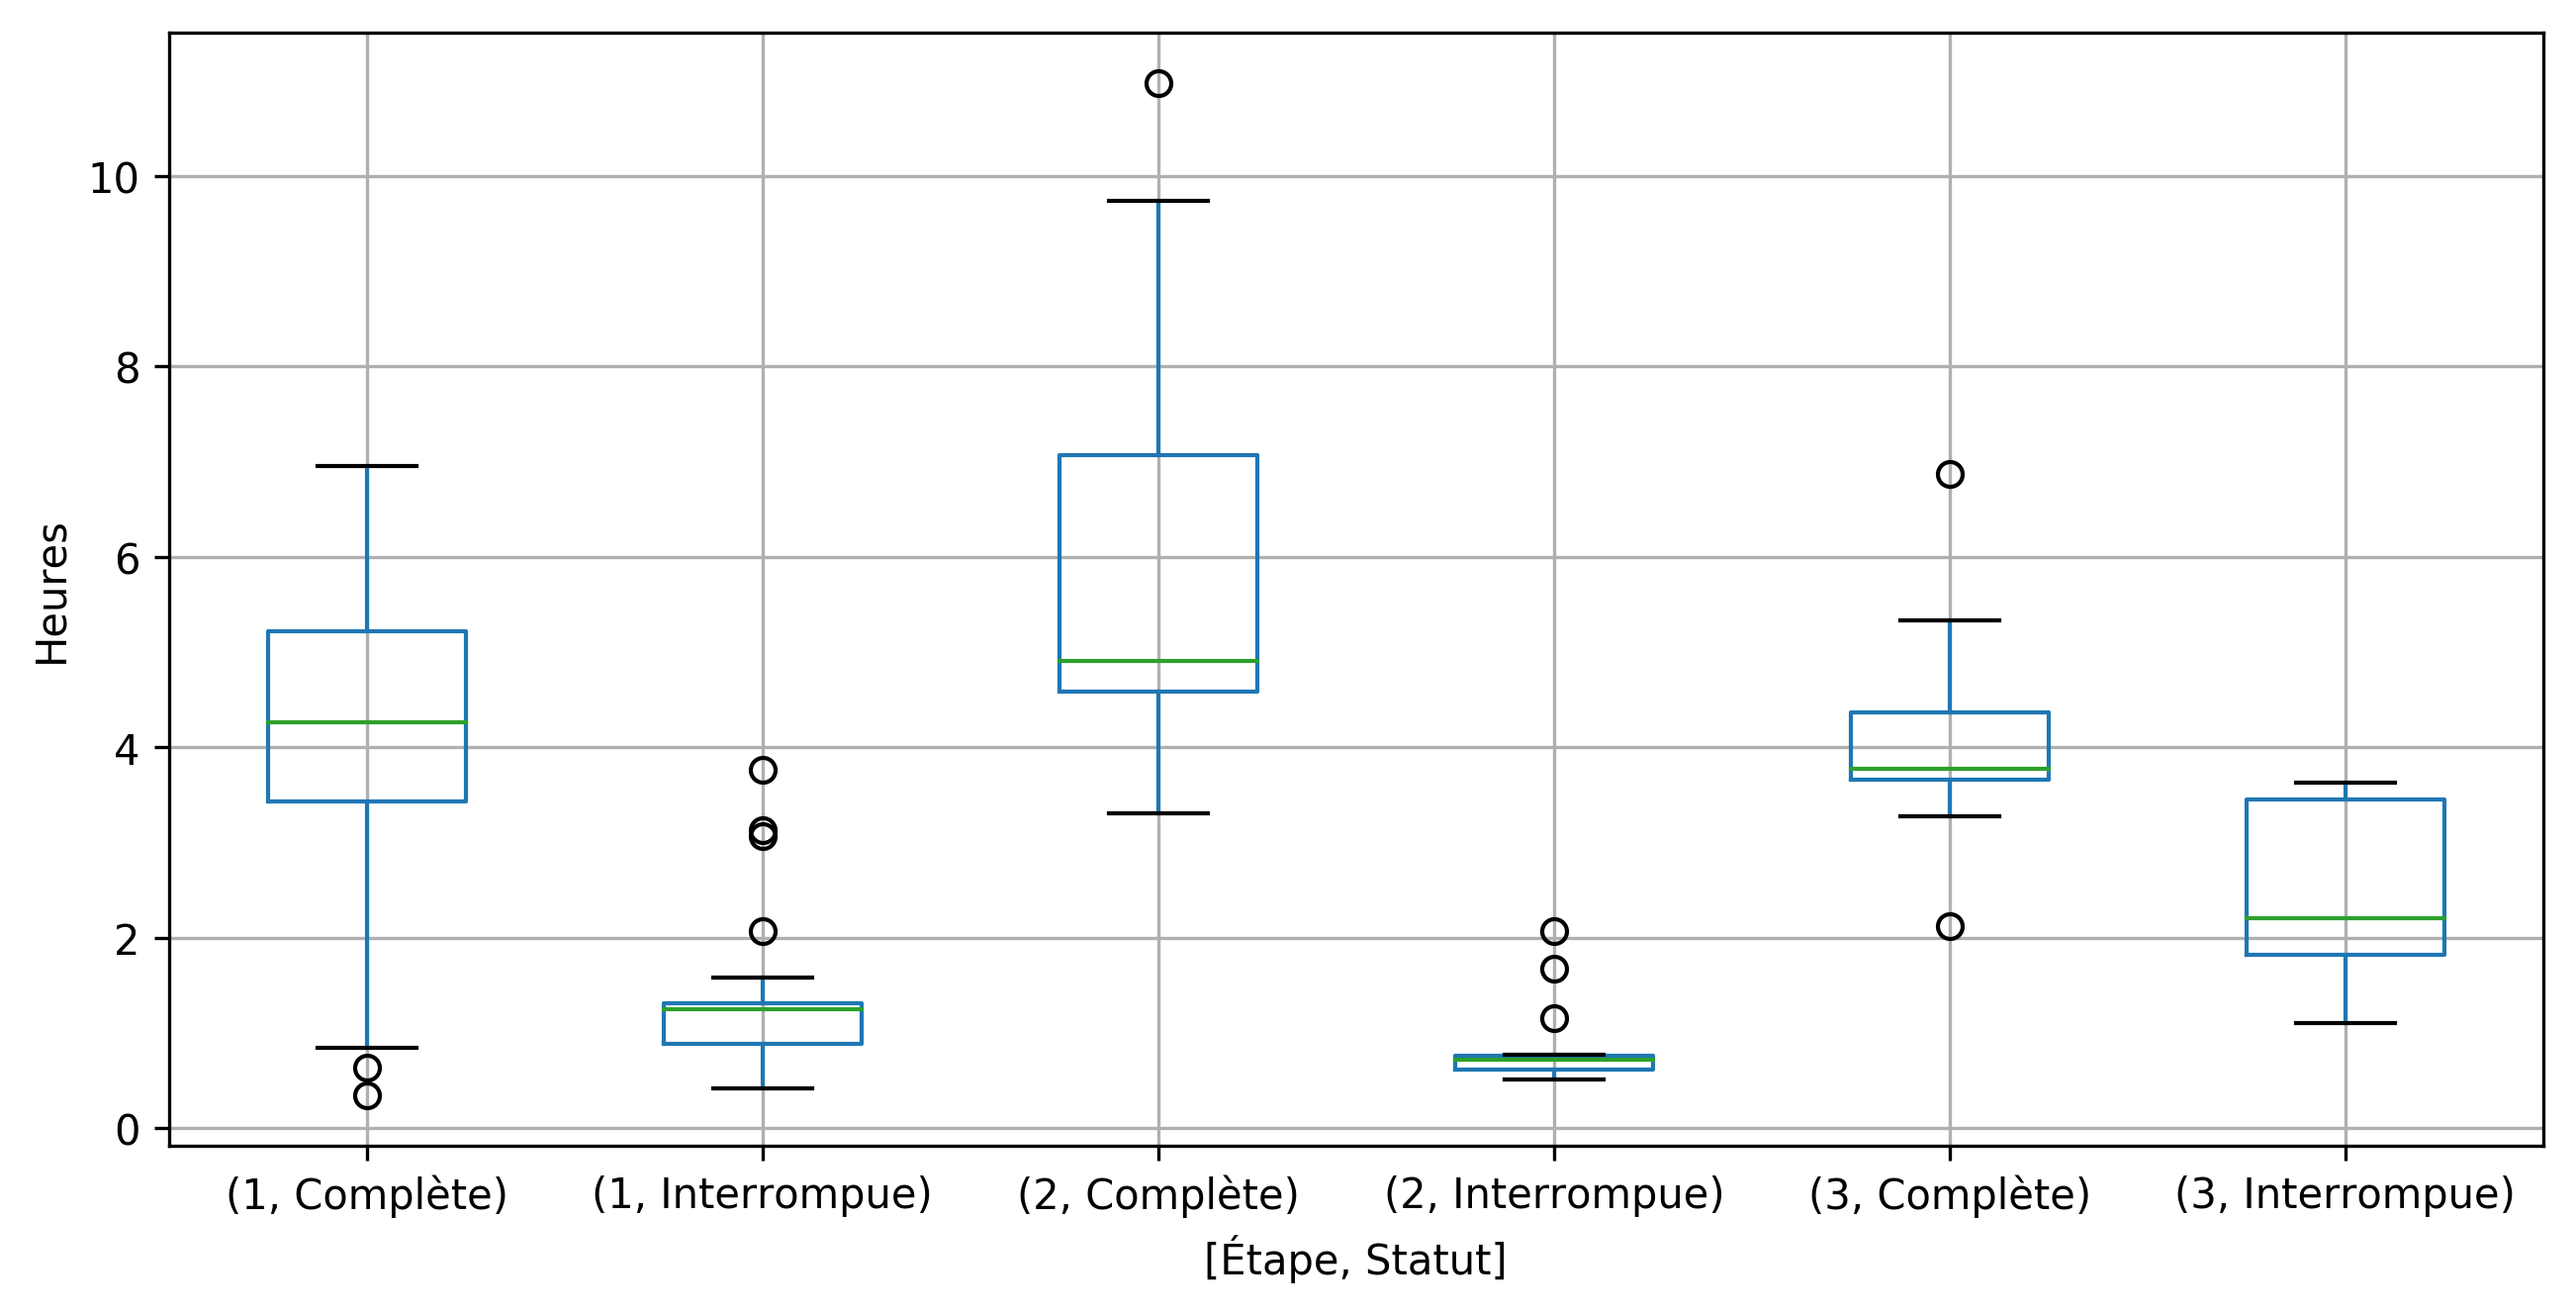
\includegraphics[width=\textwidth]{figures/chap3/entrainement/TrainingDuration96BoxPlot.png}
    \caption{Durée d'entraînement des modèles. Les populations sont les suivantes: (Étape 1, Complète) 50, (Étape 1, Interrompue) 44, (Étape 2, Complète) 11, (Étape 2, Interrompue) 19, (Étape 3, Complète) 11, (Étape 3, Interrompue) 10.}
    \label{fig:lemmatisationTrainingTime}
\end{figure}

Une fois le corpus généré, on peut lancer l'entraînement. Mais \textit{pie} comporte 97 paramètres dont 13 sont des paramètres d'architecture et 18 des paramètres d'optimisation. E. Manjavacas nous avait dans un premier temps fourni des paramètres qui lui semblaient corrects, mais nous avons souhaité vérifier leur optimisation. Dans ce cadre, nous avons utilisé deux méthodes. La première est manuelle et consiste à vérifier quelques paramètres, en particulier ceux hypothétiquement clefs, à savoir les dimensions de réseaux et le nombre de couches d'encodage des caractères ou des contextes qui déterminent en partie la capacité à apprendre du réseau. Cette méthode a eu l'avantage de nous permettre de confirmer l'identification de ces paramètres clefs et de prendre en main ces configurations. Puis, la deuxième évaluation fut réalisée avec un outil d'optimisation des hyperparamètres, \textit{optuna}\footcite{optuna_2019}, en trois phases. D'abord, l'identification des paramètres ayant le plus d'impact sur l'apprentissage: cela aura permis d'identifier sur 94 entraînements qu'avant tout autre paramètre, les \textit{learning rates} et éléments de \textit{patience} (délais avant de réduire le \textit{learning rate} ou d'estimer qu'il n'y a plus d'amélioration possible) et de prévention du surapprentissage (\textit{dropout}, ou perte volontaire d'information) ont un impact majeur sur les résultats\footnote{On peut retrouver dans les annexes numériques les trois configurations: étape 1 config-optim-base-optuna.json, étape 2 config-optim-random-optuna.json et enfin config-optim-hidden-optuna.json.}. L'étape 2 a construit sur les meilleurs paramètres de \textit{learning rate} pour évaluer les paramètres d'entraînement. Enfin, une dernière étude a été faite sur la taille optimale de la couche contexte. Ce travail est assez particulier pour le domaine des lettres, car il implique des délais pour obtenir des résultats d'expérience qui ne sont pas pas familiers à la recherche en sciences humaines: en fonction de la complexité de l'architecture, il faut compter jusqu'à 10h d'entraînement (cf. Figure \ref{fig:lemmatisationTrainingTime}) et donc plusieurs jours voire semaines pour l'évaluation simple des meilleurs paramètres\footnote{Les trois étapes cumulées représentent 17 jours et 8 heures de calcul sans interruption.}.


\subsubsection{Résultats et Variance}

Une fois les paramètres supposément optimaux trouvés, on peut lancer une batterie d'entraînements, \textit{a minima} 5, sur cette configuration et évaluer les résultats. En effet, un entraînement de \textit{machine learning }est particulièrement influençable par des phénomènes aléatoires, liés à l'initialisation des paramètres et poids, à l'ordre d'apparition des mots, etc., et peut représenter une aberration statistique. Pour l'expérience d'optimisation manuelle, on obtient une médiane des écarts-types à 0,10\% et une moyenne à 0,13\%: sur 18 configurations, on peut donc estimer qu'en moyenne, les résultats de tests seront dispersés à 0,13\% du score moyen. Dans le cadre d'un modèle performant en moyenne à 97,5\%, et à titre d'exemple, cela signifie donc que le modèle peut potentiellement avoir des résultats s'étirant de 97,35\% et 97,65\% sur plusieurs entraînements.

\begin{figure}[ht]
    \centering
    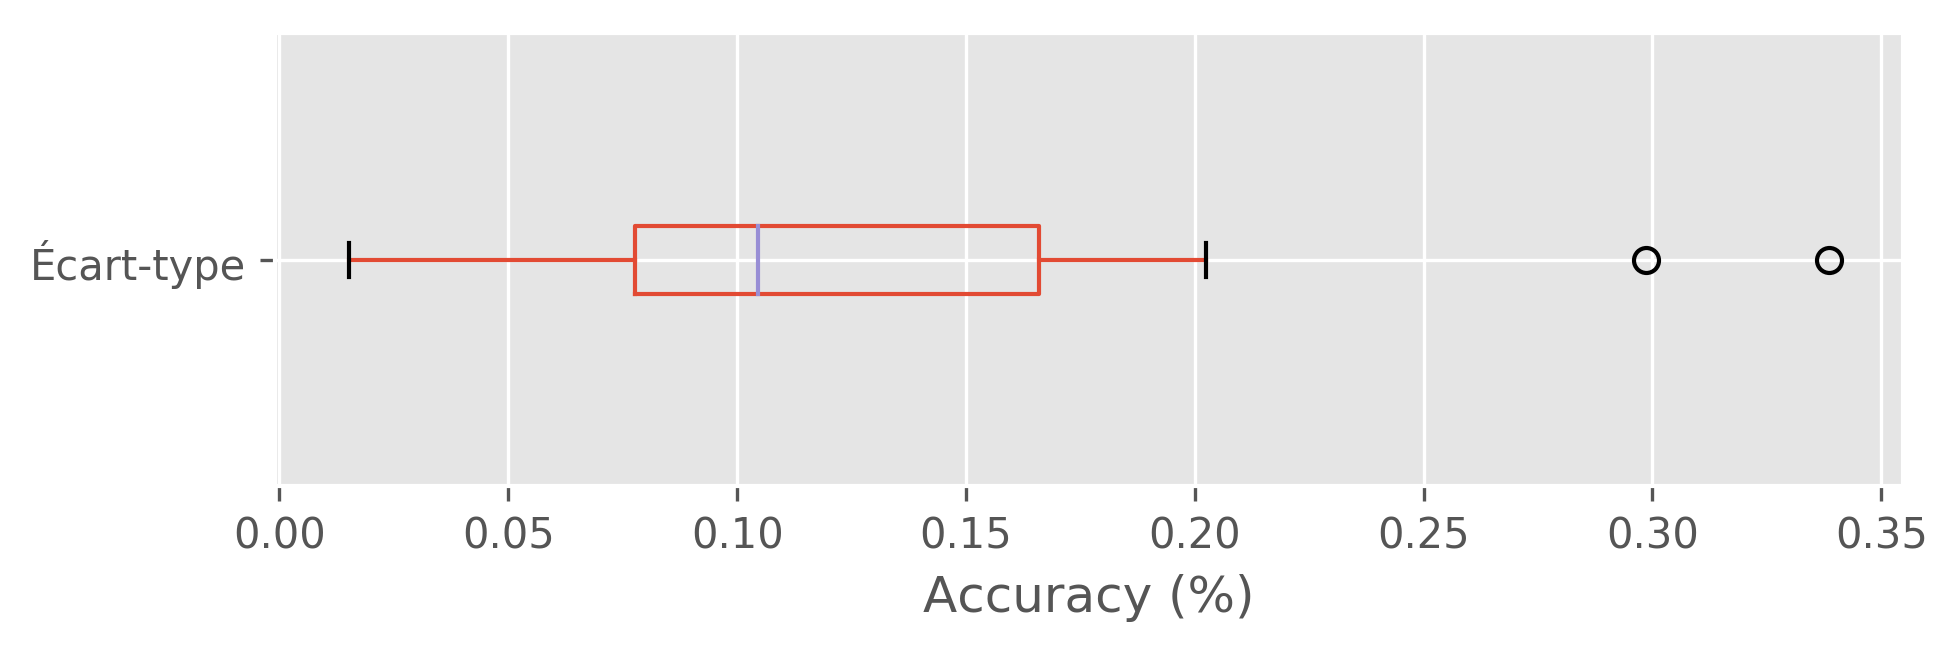
\includegraphics[width=0.7\textwidth]{figures/chap3/entrainement/Variance.png}
    \caption{Distribution des écarts-types d'\textit{accuracy} sur la tâche lemme pour 18 configurations de modèles d'entraînement sur 5 entraînements chacun. On estime alors que les modèles peuvent se retrouver, en cas de distribution parfaite, dans une intervalle de résultats d'environ 0,3\%. Pour plus de détails, \textit{cf.} figure \ref{fig:training_variation_per_model} en annexe.}
    \label{fig:training_variation}
\end{figure}

Avec la dernière configuration, le modèle obtient un score de 97,41\% en lemme sur le corpus de test et de 88,45\% sur les formes inconnues (cf. Table \ref{tab:modelFinalLemmatisation}). Les modèles d'annotations de traits morphosyntaxiques fonctionnent tous particulièrement bien, avec la tâche \texttt{cas} en queue qui plafonne à 92,34\%. En agrégeant les résultats, c'est-à-dire en prenant en compte la validité de l'ensemble des annotations automatiques (lemme, traits morphologiques, POS), on obtient les scores de 85,86\% et de 76,68\% sur les formes connues et inconnues. Ces scores sont plus bas, mais ne changent pas les conclusions précédentes: d'abord, car l'ensemble des tâches ne nous intéressent probablement pas (par exemple le degré ne devrait pas apporter beaucoup à notre travail), ensuite, car le modèle reste très performant, 85,86\% étant particulièrement élevé, surtout sur 169~000 tokens de tests. Par ailleurs, avec ses 85,86\%, le modèle n'est pas si loin des scores les plus bas, à savoir le cas (-7 points au total, -2 points sur les formes qui portent ce trait morphologique) et est infiniment plus haut qu'une probabilité de hasard parfait.

\begin{table}[ht]
    \begin{tabular}{l|rrr}
    \toprule
                    & \multicolumn{3}{l}{Accuracy}                           \\
                    & Formes connues & Formes Inconnues &  Formes Concernées \\ \midrule
    Lemme           & 97,41          & 92,92            &                    \\
    POS             & 96,49          & 92,45            &                    \\
    Genre           & 96,28          & 91,49            &   89,98            \\
    Nombre          & 97,02          & 93,85            &   96,44            \\
    Cas             & 92,34          & 87,37            &   87,84            \\
    Degré           & 98,07          & 93,96            &   93,37            \\
    Mode Temps Voix & 98,35          & 90,80            &   94,44            \\
    Personne        & 99,71          & 98,15            &   98,49            \\ \midrule
    Tâches agrégées & 85,86          & 76,68            &                    \\ \bottomrule 
    \end{tabular}
    \caption{Résultats du modèle final. Les formes concernées sont les formes dont le trait morphologique n'est pas absent: par exemple, l'\textit{accuracy} de 87,84\% en cas correspond au taux de succès pour toutes les formes qui sont annotés pour ce trait morphologique, excluant les formes verbales non participiales, les prépositions, etc.}
    \label{tab:modelFinalLemmatisation}
\end{table}

En fin d'expérimentation, un nouvel algorithme chargé de conduire l'apprentissage d'un réseau neuronal (appelé optimiseur), \textit{Ranger}\footcite{wright_new_2019} a attiré notre attention. Accompagné d'un autre système de contrôle du \textit{learning rate} qu'une réduction après rencontre de plateau\footnote{Seule option disponible de \textit{pie} au moment de cette découverte.}, \textit{CosineAnnealing}, il proposerait de meilleurs résultats que les deux grands optimiseurs que sont \textit{Adam} et \textit{SGD} (disponibles par défaut dans \textit{pie})\footnote{Nous utilisons le conditionnel ici, car, au moment de la rédaction, aucune publication vérifiée par les pairs n'était disponible sur le sujet.}. Nous implémentons donc à la fois \textit{Ranger}, \textit{CosineAnnealing} et une surcouche permettant d'imposer un délai sans optimisation du \textit{learning rate} que conseille aussi le créateur de \textit{Ranger} et faisons quelques expériences sur les paramètres\footnote{Les paramètres les plus performants rencontrés sont 0,01 de \textit{learning rate}, 10 de délai, 40 de \textit{T\_0} pour \textit{Ranger}}.Après celles-ci, il s'est avéré que l'usage de ces nouveaux algorithmes permettait non seulement de réduire le temps d'entraînement d'environ 40\%, mais aussi de stabiliser les résultats en réduisant la variance tout en obtenant de meilleurs scores\footcite{clerice_allow_nodate} (\textit{cf.} \ref{fig:lemmatisation:optimiseur:ranger}). Cette modification de notre méthode d'entraînement permet ainsi de tirer le meilleur du réseau tout en réduisant le temps nécessaire à des ré-entraînements en cas de modification du corpus.


\begin{figure}[ht]
    \hspace*{-0.05\linewidth}
    \begin{minipage}[c]{0.55\linewidth}
        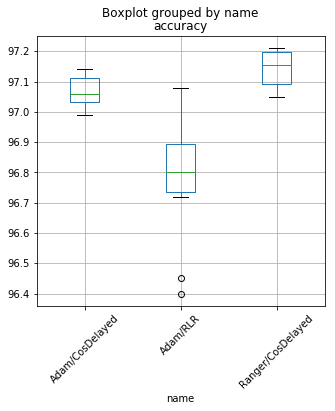
\includegraphics[width=1\linewidth]{figures/chap3/entrainement/boxplot_accuracy_ranger.png}
    \end{minipage} \hfill
    \begin{minipage}[c]{0.55\linewidth}
        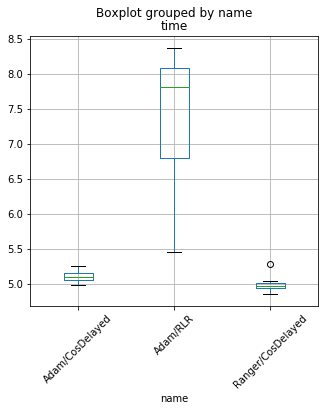
\includegraphics[width=1\linewidth]{figures/chap3/entrainement/boxplot_time_ranger.png}
    \end{minipage}
    \caption{Comparaison des résultats en fonction des optimiseurs, en temps (heure) et en \textit{accuracy}, sur trois couples: \textit{Adam/RLR} étant le système de base de \textit{pie}, \textit{Adam/CosDelayed} utilisant Adam avec un délai d'utilisation de \textit{CosineAnnealing}, Ranger/CosDelayed reprenant ce système avec \textit{Ranger} à la place d'\textit{Adam}. }
    \label{fig:lemmatisation:optimiseur:ranger}
\end{figure}

\subsubsection{Vers une typologie des erreurs}

À la suite de nos entraînements, le modèle produit est évalué sur un jeu de données de test. Ce dernier n'a pas été vu pendant l'entrainement, et garantit donc autant que possible la qualité des résultats et l'absence de surapprentissage sur le corpus d'entraînement. Suite au test, une table des confusions est mise à disposition par \textit{pie} (ex. \ref{lemma:confusion-table}). Cette table permet de mieux comprendre les différentes erreurs que le modèle est capable de faire. Pour un résultat de 97,41\% sur le corpus de test, il reste 4~395 erreurs. Sur ces erreurs, nous avons des problèmes de lemmes homographes tels que \textit{liber} et \textit{Liber}, mais aussi de pluriels lexicalisés tels que \textit{liberi}. Sur 64 apparitions dans le corpus de test de \textit{liber}, on obtient une précision de 92\% et un rappel de 89\%; pour \textit{liberi} et ses 67 apparitions on retrouve respectivement 91\% et 96\%. \textit{liber} l'adjectif est confondu 6 fois avec \textit{liberi} la substantivation et 1 fois avec \textit{Liber} la divinité, à l'inverse, \textit{liberi} est confondu 2 fois avec \textit{liber} et 1 fois avec \textit{Liber}. Si l'erreur \textit{liberi}/\textit{liber} est excusable - on peut même se demander s'il s'agit d'une erreur - on retrouve par ailleurs de vraies erreurs, avec des créations lexicales telles que \textit{pancoristus} à la place de l'attendu \textit{panchrestus} pour la forme \textit{panchresto}. Ce type d'erreur peut être introduit par un bruit involontaire créé par des formes de lemmes étymologiques qui induisent des variations orthographiques comme on en trouve avec \textit{negligens} plutôt que \textit{neglegens} et \textit{paedico} à la place de \textit{pedico}\footnote{Dans le \textit{Forcellini}, on trouve l'explication de l'orthographe sous la formule \enquote{\textit{Prima syllaba sine diphthongo scribitur vitio serioris aevi}} (la première syllabe est écrite sans diphtongue à cause du vice de la période tardive) en citant les orthographes supposées erronées des \textit{Priapea}, mais celles correctes de Catulle (21.4) et Martial (11.94.6, 11.104.17, 7.67.1, 11.99.2). Seulement, aucune des éditions modernes à notre disposition ne donne cette version en \textit{-ae-}, à savoir les éditions de Lindsay (Oxford University Press, 1929) et de Shackleton (Teubner, 1990) pour Martial, de Lafaye (Budé, 1923), de Hermman (Latomus, 1957, p. 103), de Mynors (Oxford Classical Texts, 1958) voire même la \textit{Teubner} de Mueller (1892) pour Catulle. Une recherche sur le \textit{Eagle Inscriptions Search Engine} donne deux attestations en \textit{paedic-}, une au \textit{-a-} restitué, une dont les sources (EDR et EDH) donnent une autre orthographe que celle fournie par Eagle. Au contraire, sur l'EDCS, 66 résultats (certains sont des doublons) donnent la forme \textit{pedic-}, dont le graffiti pompéien CIL 04, 10693 antérieur donc à Martial. S'il s'agissait d'une vraie diphtongue, cette chute de la prononciation de la diphtongue pourrait avoir eu lieu avant Cicéron, \textit{cf.} \cite{sturtevant_monophthongization_1916}. L'autre hypothèse ici est celle d'une étymologie grecque supposée par des lexicographes qui auraient archaïsé de ce fait la forme du lemme.}. Si ce type d'erreur existe pour le couple \textit{liberi}/\textit{liberi}, on peut par ailleurs, par un croisement avec les données de collatinus, remarquer que:

\begin{enumerate}
    \item 5,54\% des erreurs sont des lemmes verbes remplacés par leur participe parfait passif et donc une forme adjectivale lexicalisée (type \textit{beo}/\textit{beatus})
    \item 5,57\% sont des verbes remplaçant la forme adjectivale, l'inverse de la situation 1.
    \item 1,16\% sont des verbes dont le participe présent rentre en collision avec le lemme attendu (type \textit{negligens}/\textit{negligo}).
    \item 0,96\% sont des erreurs inversées de 3.
    \item 3,59\% sont des noms partageant leur nominatif avec une forme adjectivale (\textit{liberi}/\textit{liber}).
    \item 6,76\% sont des erreurs inversées de 5.
    \item et enfin, 0,50\% des erreurs sont des verbes passifs lemmatisés en actifs, et 0,66\% correspondent à l'inverse.
\end{enumerate}

\begin{table}[]
\centering
\begin{tabular}{lrlr}
\toprule
Expected & Total Errors & Predictions & Predicted times \\ \midrule
qui      & 289          & quod        & 111             \\
         &              & quis        & 103             \\
         &              & quam        & 39              \\
         &              & quo         & 24              \\
         &              & qua         & 11              \\
         &              & quiuis      & 1               \\
quis     & 174          & qui         & 156             \\
         &              & quo         & 8               \\
         &              & quam        & 5               \\
         &              & quod        & 3               \\
         &              & qua         & 1               \\
         &              & cuius       & 1               \\
quod     & 108          & qui         & 103             \\
         &              & quis        & 5               \\
multus   & 56           & multum      & 37              \\
         &              & multi       & 19              \\
bonus    & 26           & bonum       & 14              \\
         &              & bene        & 8               \\
         &              & boni        & 3               \\
         &              & Bonus       & 1               \\ \bottomrule
\end{tabular}
\caption{Table des confusions générée par \textit{pie}. Nous retenons pour l'exemple les confusions en lemme les plus fréquentes.}
\label{lemma:confusion-table}
\end{table}

Dans un cadre plus large, sur 4~398 erreurs, 2~942 portent sur des tokens ambigus, connaissants donc plusieurs solutions de lemmatisation, soit 8,08\% de ceux-ci. 451 erreurs portent sur des lemmes inconnus en phase d'entraînement, soit 40\% de ces derniers, mais le faible nombre de ceux-ci ne permet pas d'en tirer de vraies analyses statistiques.

\section{Pie: extensibilité des résultats}

L'entraînement de \textit{pie} sur un corpus test donné nous informe de sa valeur sur le corpus en tant que tel. Se pose la question cependant de la capacité de nos modèles à s'appliquer à un corpus étranger, de quantifier l'impact d'une potentielle spécialisation. Pour étudier cet impact, nous proposons quatre expériences qui permettront d'évaluer l'impact de la taille du corpus d'entraînement, de sa variété en style et en genre, et enfin une étude hors-domaine s'appliquant d'abord à un texte important pour notre corpus, les \textit{Priapea}, puis à des extraits de textes tardifs, le corpus du LASLA s'arrêtant avant la fin du premier siècle de notre ère..

\subsection{Évaluation sur des données hors domaine}
\label{subsec:lemmatisation:hors-domaine}

Si les tests du modèle nous présentent un outil performant, au-delà des 97\% de reconnaissance des lemmes, ils ne nous montrent qu'une face de son usage. En effet, la constitution du corpus de test est faite d'extraits non connus certes, mais d'extraits des mêmes textes que le corpus d'entraînement. Ils ont donc une très forte probabilité de posséder les mêmes caractéristiques en termes de syntaxe, de vocabulaire, de coupes opérées par l'éditeur. Par ailleurs, ils posent un second problème qui est celui de la période couverte par le corpus d'origine, à savoir que l'auteur le plus tardif dans le corpus est Juvénal (127\footcite[p. 320]{zehnacker_litterature_2013}), puis Sénèque (65\footcite[p. 231]{zehnacker_litterature_2013}). Ces données quand elles sont issues du même corpus, qu'elles sont des fractions des mêmes textes que les corpus d'entrainement et de \textit{dev} sont appelées \enquote{en domaine} (\textit{in domain}).

Au contraire, on parle en apprentissage machine de données hors domaine, des données dont les traits de définitions (auteur, genre, période, style, œuvre, etc.) diffèrent pour tout ou partie des données d'entraînement. Pour cette étude, nous proposons deux corpus hors domaines, l'un constitué de l'ensemble des priapées 1 à 78 d'après la numérotation de Baehrens, l'autre constitué de 10 textes d'auteurs tardifs, majoritairement chrétiens. Les \textit{Priapea} offrent un texte à l'extrême fin de notre corpus en termes de chronologie\footcite{citroni_les_2008} et sont parmi les œuvres non étiquetées les plus portées sur le sexe. Par ailleurs, le style court tout particulier de cet ouvrage offre aussi un grand nombre de sujets différents sur un corpus finalement assez réduit (environ 3~000 mots). Le second corpus\footcite{glaise_2020_corpus_tardif} est constitué d'échantillons de dix-neuf œuvres de dix-sept auteurs, dont les passages (hors ponctuation) comptent \textit{a minima} 500 mots et dont les auteurs s'étendent du deuxième siècle au neuvième de notre ère (Eginhard) avec une concentration plus forte autour du quatrième (cf. \ref{corpus:glaise:dates}). Si la date de fin de ce corpus est plus tardive que les bornes que nous nous sommes posées, elles permettent d'évaluer tout de même la capacité du modèle à s'étendre dans le temps malgré un entraînement spécifique sur un corpus allant de la république au Haut-Empire, où les marques de la chrétienté sont de fait absentes.

\begin{table}[h]
\centering
\begin{tabular}{l|rrrrrrr}
\toprule
Siècle           & 2 & 3 & 5 & 6 & 7 & 7 & 9 \\ \midrule
Nombre d'auteurs & 1 & 3 & 5 & 4 & 2 & 1 & 1 \\
Nombre de textes & 2 & 3 & 6 & 4 & 2 & 1 & 1 \\ \bottomrule
\end{tabular}
\caption{Répartition par siècle des auteurs et œuvres du corpus Glaise}
\label{corpus:glaise:dates}
\end{table}

\subsubsection{Résultats généraux}

Le modèle propose des résultats convaincants sur une très grande majorité des \textit{Priapea}. La particularité de cette œuvre tient, d'un point de vue statistique, à leur très petite taille: une médiane à 30 mots sur les soixante-seize premiers poèmes et une moyenne à 40 à cause d'individus aberrants tels que le poème 51 (150 mots) et 68 (237)\footnote{Au niveau des quartiles, 25\% des \textit{priapées} font moins de 24 mots, 75\% en font moins de 68. Toutes les tailles ne concernent que les mots, hors ponctuation donc, mais incluant les clitiques.}. L'\textit{accuracy} peut donc grandement varier d'un texte à l'autre, une erreur pouvant représenter au pire une chute de 9\% d'un score\footnote{C'est le cas potentiellement des priapées 13, 59 et 62 dans notre édition.} ou au mieux 0,4\% pour la plus grande priapée. Les résultats restent plus qu'honorables, avec une baisse d'uniquement trois points par rapport au corpus de test principal et une accuracy globale de 94,2\% sur la tâche de lemmatisation (\textit{cf.} table \ref{tab:out_of_domain_global_accuracy} et figure \ref{fig:priapea_varations_boxplot}). Certaines priapées ont des scores particulièrement bas qui ne semblent pas avoir de lien avec leur taille: on notera ainsi les priapées 75 (82 mots, 84\%) et 46 (45 mots, 84\%) qui se trouvent dans la moyenne haute des tailles de poème.

Comme le corpus des \textit{Priapea}, le corpus de latin tardif propose des résultats avec une faible perte, de l'ordre de trois points aussi. L'ensemble des autres annotations performent globalement mieux que sur les \textit{Priapea} (annotation \textit{cas} à 92,9\% contre 89,4\%) ce qui peut potentiellement s'expliquer par la forme poétique et courte des poèmes qui ne laisse pas une grande place à l'erreur. Dans ce corpus, deux textes font office de résultats aberrants, à savoir Jérôme, \textit{In Hieremiam} et Grégroire de Tours, \textit{Historia Francum} qui chutent respectivement à 87 et 88\%. Les textes ont majoritairement la même taille, aux alentours de 500 à 600 mots, avec Commodien, \textit{Instructiones} comme texte le plus court (412 mots) et Augustin, \textit{De Civitate Dei} ainsi que Hilaire de Poitiers, \textit{Tractatus super psalmos} comme textes extrêmement longs\footnote{L'export des textes à corriger ayant allongé les textes involontairement, et l'annotation ayant été corrigée, l'ensemble de ces textes a tout de même été conservé, produisant de fait un écart avec la moyenne de 500 mots.}.

\begin{table}[h]
    \centering
    \begin{tabular}{l|rr|rr}
    \toprule
         Catégorie &  \multicolumn{2}{c}{\textit{Accuracy}} & \multicolumn{2}{c}{\textit{Accuracy} quand applicable} \\
    \midrule    
                {} &  Priapées &    Tardif                  & Priapées &    Tardif                                   \\
    \midrule
             lemma &     94,2 &    94,5                   &   N/A    &    N/A                                      \\
               Deg &     96,8 &    97,5                   &   90,3   &    91,5                                     \\
              Numb &     94,7 &    96,5                   &   94,1   &    96,4                                     \\
            Person &     99,0 &    99,7                   &   96,0   &    99,1                                     \\
Mood\_Tense\_Voice &     96,1 &    97,7                   &   87,0   &    92,3                                     \\
              Case &     89,4 &    92,9                   &   84,1   &    88,0                                     \\
              Gend &     91,7 &    92,8                   &   77,8   &    79,2                                     \\
               pos &     95,0 &    67,6                   &   N/A    &    N/A                                      \\
    \bottomrule
    \end{tabular}
    \caption{Résultat du modèle sélectionné sur le corpus des priapées et de latin tardif. L'accuracy quand applicable désigne la précision de l'algorithme sur les termes qui nécessitent une annotation, en d'autres termes, pour la personne par exemple, seules les annotations sur les verbes sont concernées.}
    \label{tab:out_of_domain_global_accuracy}
\end{table}


\begin{figure}[ht]
    \centering
    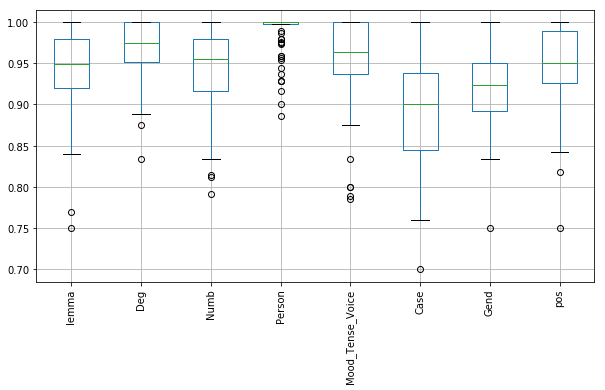
\includegraphics[width=0.7\linewidth]{figures/chap3/extensibilite/PriapeaBoxPlot.png}
    \caption{Variation des taux d'erreur sur l'ensemble du corpus des \textit{Priapées}}
    \label{fig:priapea_varations_boxplot}
\end{figure}

\subsubsection{Étude des erreurs}

Si ces chiffres annoncent potentiellement une très bonne nouvelle pour la période tardive et les sujets qui nous intéressent, ne s'attarder que sur l'échelle quantitative macro serait une erreur de taille: 6\% de réponses fausses laissent possible un très grand nombre d'erreurs dont il faut avoir conscience. D'abord, parce que dans un contexte traditionnel de richesse lexicale, la loi de Zipf se retrouvant logiquement dans chacun des corpus, on sait que les termes les plus fréquents représentent une très grosse partie du corpus final. Sur le corpus latin tardif, sur 15~188 formes, 4~908 formes dépendent de 34 lemmes qui apparaissent au minimum plus de 100 fois\footnote{Il s'agit du quantile 0,99 du corpus.}. Parmi ces lemmes, seuls 3 sont des verbes (\textit{sum}, \textit{dico}, \textit{facio}) et 3 des noms communs (\textit{deus}, \textit{dominus}, \textit{filius}); seuls les noms présentent une particularité thématique, les trois verbes étant particulièrement fréquents dans la langue latine en général. Il est fort peu probable que des erreurs arrivent sur des termes comme \textit{de}, \textit{pro} ou encore \textit{ab}. Ensuite, parce que notre corpus tardif global représente au moins la moitié de notre corpus latin pris en compte dans nos recherches, et que l'on ne saurait alors se satisfaire d'une inconnue aussi importante.

Dans un premier temps, nous proposons de regarder quelles POS posent un problème au lemmatiseur. Dans un contexte de distribution normale, une POS représentant 40\% des POS du corpus devrait posséder 40\% des erreurs. Or, en figure \ref{fig:latin_tardif_error_pos}, on remarque nettement que les noms propres (NOMpro) ont une très nette surreprésentation parmi les erreurs, avec des cas extrêmes de plus de 50\% des points d'\textit{accuracy} perdus, mais moins de 5\% des mots du corpus. Si l'on prend un corpus type de 500~mots, et 94\% de succès, on dénombre pour ces cas extrêmes 25 noms propres (5\% du corpus), 30 erreurs (6\% d'erreurs) dont 16 ou 17 sont des noms propres. Pour mesurer cet écart, on propose une mesure $Impact$ définie telle que $\text{Impact}_{pos} = \frac{\text{Erreurs}_{pos}}{\left | \text{Erreurs} \right |} \div \frac{\text{Tokens}_{pos}}{\left | \text{Tokens} \right |}$. Ainsi, un impact médian de 6,84 pour la POS nom propre indique que la proportion d'erreurs sur les noms propres est presque sept fois supérieure à la proportion de tokens qu'elle représente. Bien que les verbes et les noms communs aient une forte responsabilité dans le nombre d'erreurs, les médianes de leur Impact sont respectivement de 1,37. Ces impacts très légèrement supérieurs à 1 ne sont pas anormaux, tant certaines catégories ne représentent aucune erreur malgré une importante fréquence: les prépositions représentent ainsi  7\% en moyenne des corpus contre 0\% des erreurs, il en va de même pour les adverbes négatifs (14\%) et les conjonctions de coordination (7\%).

\begin{figure}
    \centering
    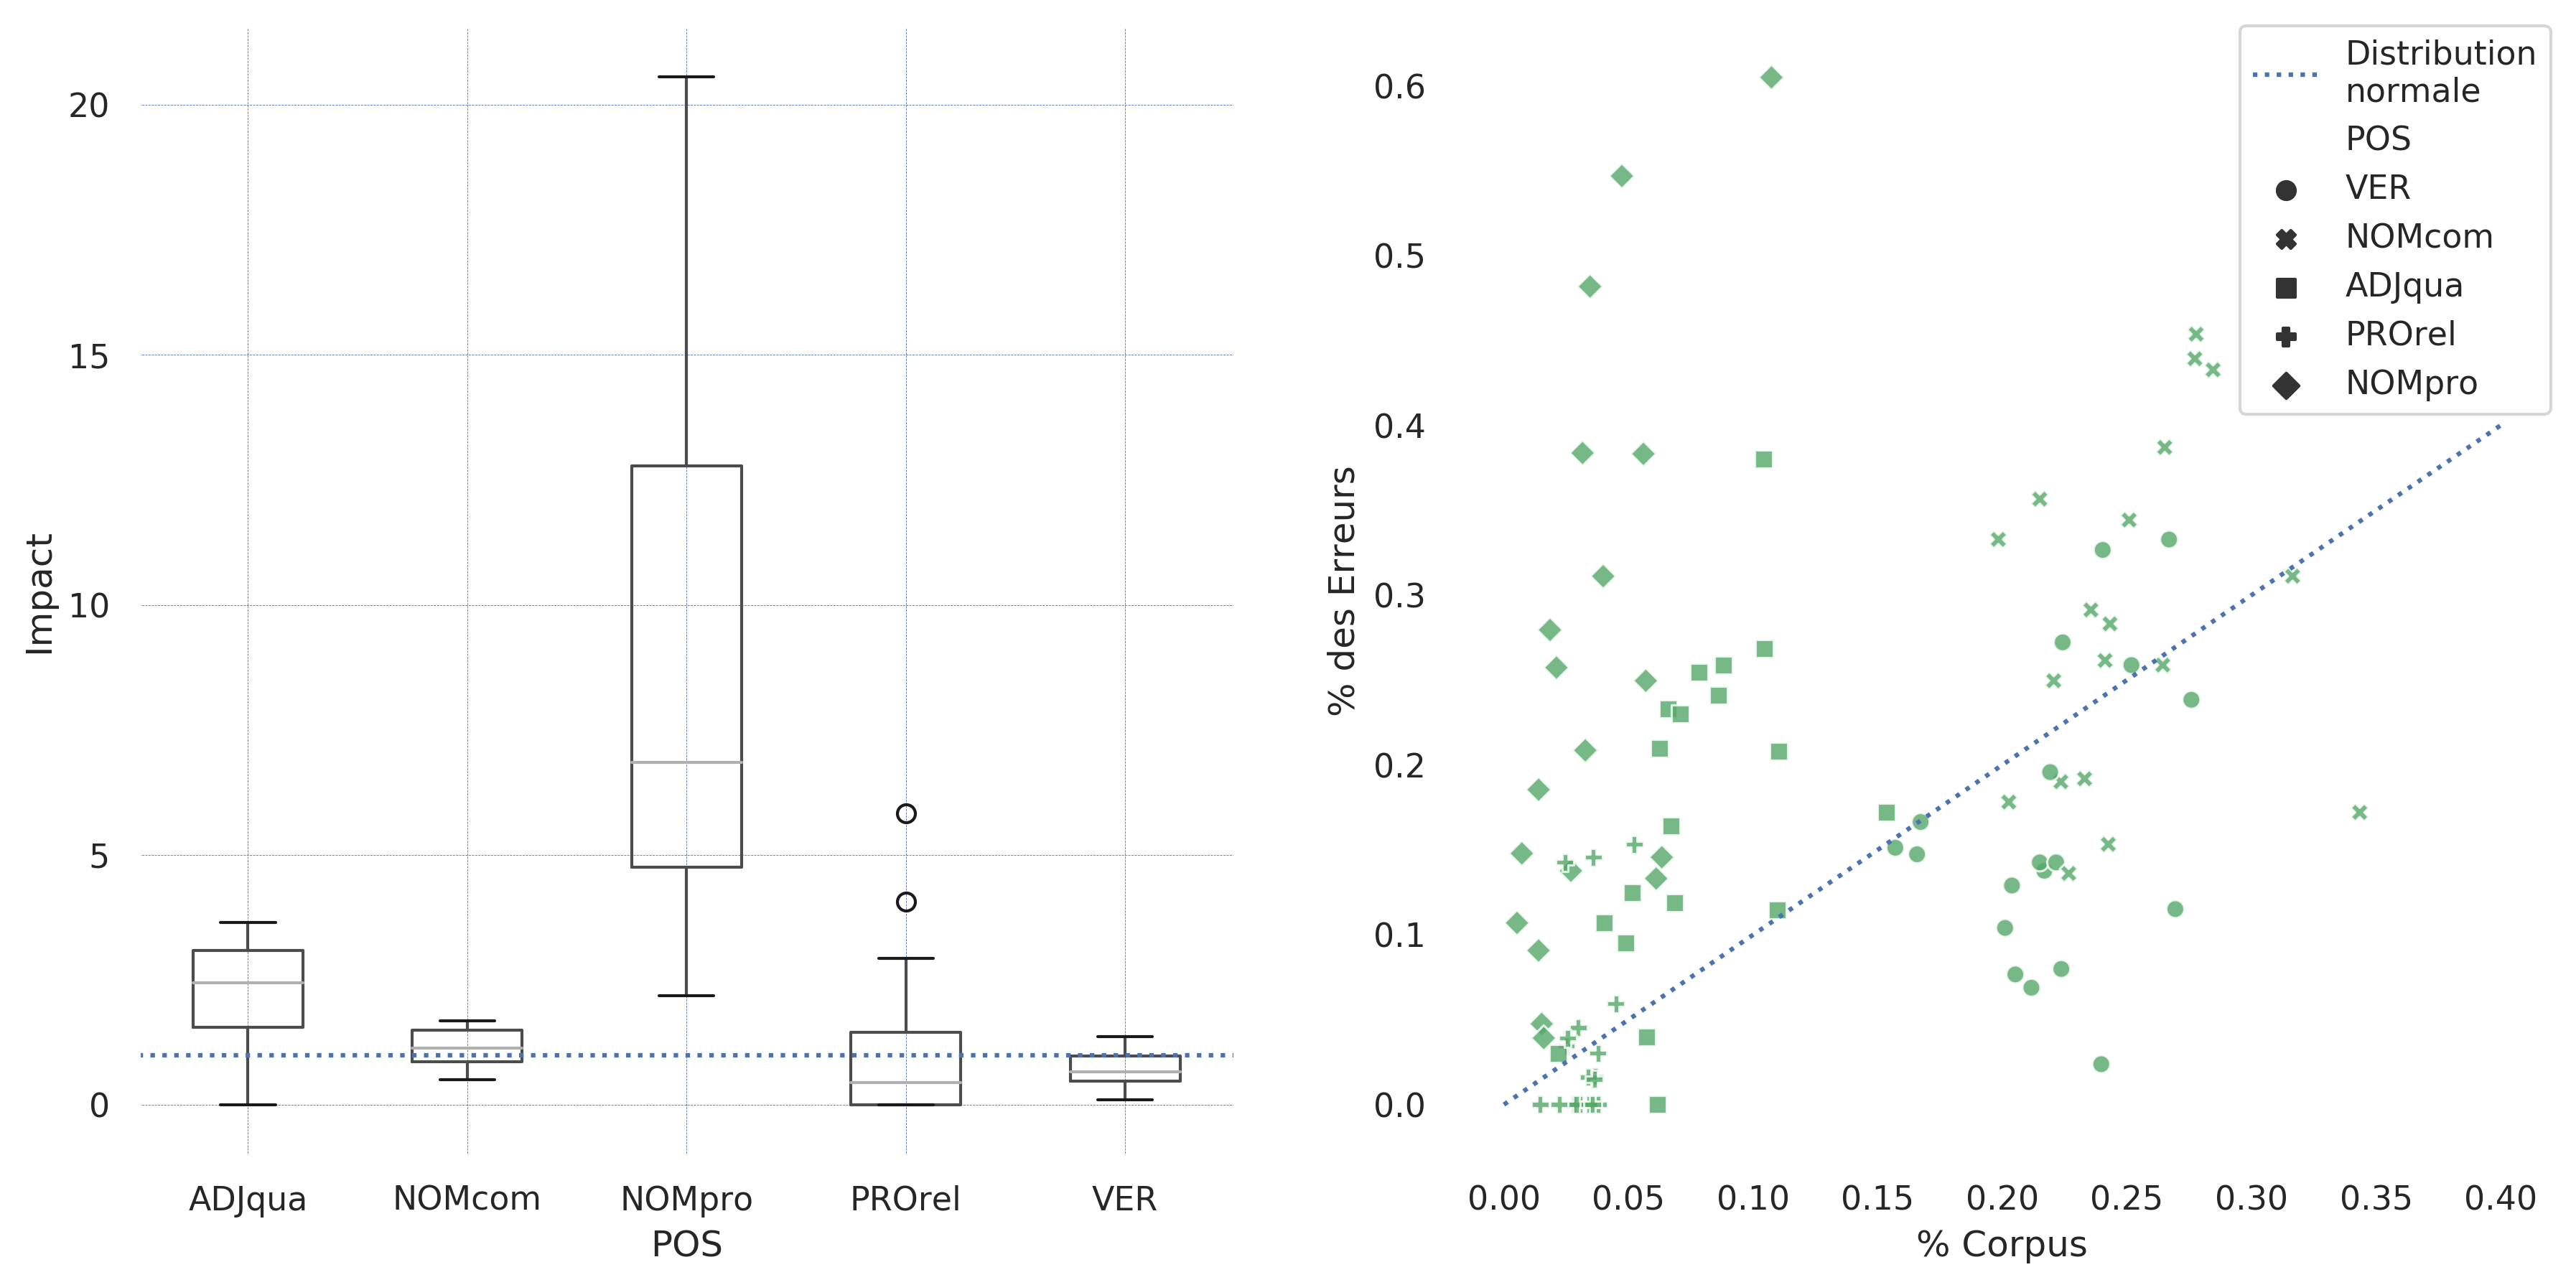
\includegraphics[width=1\linewidth]{figures/chap3/extensibilite/LatinTardifPosErrorBoxPlot.png}
    \caption{Responsabilité des POS dans les erreurs du lemmatiseur sur le corpus tardif.}
    \label{fig:latin_tardif_error_pos}
\end{figure}

Désormais, nous pouvons étudier la catégorie des noms propres de plus près. On peut classer les erreurs dans quatre grandes catégories:
\begin{itemize}
    \item Le lemme n'est pas reconnu comme nom propre, car il est vraisemblablement une personnification d'un nom commun par exemple ou bien qu'il n'est pas reconnu comme tel. On rencontre le premier cas avec \textsc{terra} à la place de \textsc{Terra}, \textsc{mater}/\textsc{Mater}, etc. et le second avec *\textsc{uenus} en place de \textsc{Uenus}, *\textsc{iesus}/\textsc{Iesus}.
    \item Le lemme est pris au pluriel à la place du singulier: c'est un problème commun sur les noms de peuples (\textsc{Graecus} contre \textsc{Graeci}).
    \item Le lemme est issu de la langue grecque ou hébraïque: \textsc{Christus}, \textsc{Israel}, \textsc{Pascha}, \textsc{Dauid}. Sur le corpus entier du LASLA, les occurrences de termes dépendant de la déclinaison grecque ne représentent que 1,1\% des noms, soit 5~585 individus sur environs 487~000. Bien que des noms d'origine grecque puissent suivre des déclinaisons latines comme Christus, on peut s'attendre à de plus grandes difficultés sur les autres termes tant ils ont été peu vus à l'apprentissage.
    \item Le lemme possède une variation graphique latine forte, chose inconnue dans le corpus classique, ainsi on trouve les couples \textit{Bethleem}/\textit{Bethlehem}, \textit{Hierusalem}/\textit{Ierusalem}, \textit{Hiezechiel}/\textit{Ezechiel}, ou encore \textit{Hadrianus}/\textit{Adrianus}.
\end{itemize}

Une fois la catégorie des noms propres analysée, on trouve, en plus de ces cas d'erreurs, les types suivants:
\begin{itemize}
    \item Une erreur sur le choix de racine, à savoir le choix entre le verbe \textit{debeo} et le nom \textit{debitum} par exemple.
    \item Une situation inverse au premier cas des noms propres, à savoir un nom commun pris pour un nom propre et dont la première lettre est ainsi capitalisée.
    \item Une erreur sur une racine reconstruite en adjectif de la première classe (en -us donc) à la place d'un nom, comme pour \textit{prophetia}/\textit{prophetius}.
    \item Un problème de lemme à l'orthographe \enquote{réactionnaire}: dans le corpus des Priapées, on rencontre plusieurs fois l'erreur \textit{pedico} contre l'orthographe \enquote{juste} \textit{paedico} du LASLA.
\end{itemize}

Ces catégories semblent couvrir une très grande partie des erreurs hors pronom et permettent d'éclairer les résultats obtenus, mais aussi de cibler les domaines où le corpus peut être amélioré ou bien là où un correcteur automatique pourrait intervenir, en ciblant par exemple les lemmes d'origine grecque ou hébraïque. Ils ne donnent cependant qu'un éclairage particulier sur le résultat du modèle, mais pas sur sa capacité d'apprentissage et de l'influence du corpus d'entraînement.

\subsection{Étude de l'impact de la taille du corpus sur l'efficacité du modèle}
\label{lemmatisation:extensibilite:tailles}

Pour la première expérience, nous voulons évaluer l'impact de la taille d'un corpus sur les différents éléments de mesure à notre disposition. Nous proposons donc des coupes du corpus LASLA à 1\%, 5\%, 7,5\%, 10\%, 20\%, 40\%, et enfin 80\%. Dans chacun des jeux d'entraînement, on réservera 10\% du résultat de la coupe pour un \textit{set} de développement. La découpe se fait au niveau de chacun des fichiers d'entraînement du LASLA, à savoir un découpage au niveau de l'œuvre (\textit{Carmina} de Catulle) ou à un sous-niveau de celle-ci (César, \textit{Bellum Gallicum}, 1). Chaque séquençage connait alors la même variété d'auteur, la même variété de genre et de thème. Les jeux formés d'extraits pris aléatoirement dans les phrases constituées par le LASLA. Nous mesurons trois tâches, à savoir:

\begin{itemize}
    \item la tâche \texttt{lemma}, qui indique une compréhension du vocabulaire, de la syntaxe et de la morphologie,
    \item la tâche \texttt{POS}, qui indique une compréhension morphosyntaxique
    \item la tâche \texttt{Gend}, qui indique une compréhension de la morphologie.
\end{itemize}

Durant l'entraînement, le modèle principal ayant obtenu les meilleurs résultats sur le corpus global a montré des faiblesses sur les corpus de petite taille. Pour chaque corpus, deux configurations ont donc été testées, une avec un module GRU simple couche (RNN=1) et un module GRU double couche (RNN=2) pour la partie de \textit{character embeddings}. Les résultats (\textit{cf.} Table \ref{tab:percent_corpus_comparaison}) montrent que l'augmentation de la taille du corpus avec une même variété de genres et d'auteurs a un impact fort (plus de 1 point de gagné) jusqu'à l'utilisation de 40 \% du corpus, quelle que soit la tâche, ou presque\footnote{Il existe en effet des valeurs aberrantes pour le genre et la POS au moment du passage de 7,5\% à 10\% du corpus.}. Au contraire, les passages de 40\% à 60\% du corpus et de 60\% à 80\% ne représentent des gains que de 0,23 et 0,46 point respectivement, et donc, un passage de 96,79\% d'\textit{accuracy} pour le corpus à 40\% à seulement 97,48\% pour celui à 80\%, pour un doublement du nombre de tokens annotés utilisés pour l'entraînement, soit une augmentation d'environ 600~000 tokens (passage de 622~238 tokens d'entraînement à 1~226~227).


\begin{table}[]
    \centering
    \resizebox{\textwidth}{!}{%
    \begin{tabular}{ll|rrrrrrrr}
    \toprule
     RNN &  \% Corpus &  Lemme &  $\Delta$(Lemme) &  $\theta$ Lemme &  $\Delta$($\theta$ Lemme) &   POS &  $\Delta$(POS) &  Genre &  $\Delta$(Genre) \\
    \midrule
       1 &     0,010 &  0,741 &     0,000 &    0,725 &       0,000 & 0,791 &   0,000 & 0,851 &    0,000 \\
       1 &     0,050 &  0,889 &     0,149 &    0,858 &       0,133 & 0,887 &   0,096 & 0,902 &    0,052 \\
       2 &     0,075 &  0,921 &     0,031 &    0,855 &      -0,002 & 0,921 &   0,034 & 0,930 &    0,028 \\
       2 &     0,100 &  0,936 &     0,015 &    0,894 &       0,039 & 0,929 &   0,008 & 0,933 &    0,003 \\
       2 &     0,200 &  0,949 &     0,013 &    0,882 &      -0,012 & 0,947 &   0,019 & 0,948 &    0,015 \\
       2 &     0,400 &  0,968 &     0,019 &    0,922 &       0,041 & 0,961 &   0,013 & 0,961 &    0,012 \\
       2 &     0,600 &  0,970 &     0,002 &    0,924 &       0,002 & 0,964 &   0,003 & 0,965 &    0,004 \\
       2 &     0,800 &  0,975 &     0,005 &    0,910 &      -0,014 & 0,966 &   0,002 & 0,970 &    0,005 \\
    \bottomrule
    \end{tabular}}
    \caption{Résultat des tests sur un corpus de test de 140~000 mots représentant 80\% du corpus de test original. RNN correspond au nombre de couches du module d'encodage des caractères. Les mesures de gain entre deux étapes, notées $\Delta$ correspondent à la différence avec le modèle précédent, il faut donc lire \enquote{Le modèle à 80\% du corpus performe 0,46 point de plus que le modèle à 60\% du corpus.}. On ajoute une mesure sur un corpus hors domaine, celui de latin tardif, que l'on désigne dans les colonnes par un $\theta$}
    \label{tab:percent_corpus_comparaison}
\end{table}

D'après ces résultats, on peut penser que le lemmatiseur apprend \enquote{assez} de la richesse de vocabulaire et de la syntaxe d'un auteur pour s'enrichir jusqu'à environ 40\% de ses textes. Une stratégie de création de corpus pourrait donc se focaliser sur l'annotation d'extraits d'auteurs, plutôt qu'une approche d'annotation complète. Cependant, on peut aussi voir les gains minimes comme de véritables bonds en valeur absolue: si, pour un corpus de 10 millions de tokens, les résultats passent de 96,09\% d'accuracy à 96,97\%, et que ces résultats se retransmettent de manière régulière, le nombre d'erreurs passe de 391~000 à 303~000, soit une chute de 88~000 erreurs. Les progressions en \texttt{POS} et en \texttt{Genre} sont toutes les deux limitées au même titre que celle de lemme. Par ailleurs, lors d'une évaluation sur le corpus de latin tardif, on se rend compte que l'extensibilité connait de grosses variations et y compris des reculs (-0,2 point, -1,2 point, -1,4 point sur les passages 5\%, 20\% et 80\%). Nous ne pouvons ici que faire des hypothèses, et deux semblent plus probables que d'autres. La première consiste à estimer qu'il y a un phénomène aléatoire sur la performance en hors domaine, et que, sur une dizaine d'entraînements, on trouverait majoritairement des modèles améliorant le score précédent. Si cette hypothèse est alléchante, elle n'en reste pas moins assez faible, surtout pour des baisses de 1,4 point en hors domaine, mais une augmentation même faible en test classique: elle serait plus crédible sur un écart de moins de 0,5 point, comme nous avons déjà pu le voir sur d'autres entraînements. La deuxième hypothèse consiste à un surapprentissage sur le corpus d'entraînement: le modèle se surspécialiserait sur le corpus classique, se rendant incapable de reconnaître le corpus tardif. Là encore cette hypothèse pose problème, car elle n'expliquerait pas pourquoi, sur un corpus à 100\%, nos scores rebondissent à plus de 94,5\% (+3 points). Il n'est cependant pas à exclure une savante combinaison des deux phénomènes qui créerait ainsi une chute des plus remarquables.



\begin{comment}
\subsection{Taille et diversité: corpus Perseus}
\label{lemmatisation:extensibilite:perseus}

Nous avons vu en \ref{subsec:treebank_corpora} que le corpus de Perseus pour le treebank, mis en forme pour le projet Universal Dependencies (\Gls{UD}), présente un corpus comprenant peu de textes et peu de mots comparés au corpus du LASLA (26 000 mots contre 1,7 million), mais cependant une variété de style et d'époques assez forte parmi les corpus de ce genre.

\newpara

Pour compléter l'analyse précédente \ref{lemmatisation:extensibilite:tailles}, on reproduit un corpus similaire à celui de Perseus, dans la limite où 4 œuvres présentes dans ce dernier ne le sont pas dans le corpus LASLA, à savoir les \textit{Fabulae} de Phèdres, les \textit{Res Gestae} d'Auguste, la \textit{Vie d'Auguste} de Suétone, la \textit{Vulgate} de Jérôme. On propose de remplacer pour le même nombre de phrases par deux autres œuvres \footnote{Ces œuvres sont mentionnées dans le corpus de Perseus original, mais n'ont pas été nettoyées pour le projet \Glspl{UD})} à savoir les \textit{Fastes} d'Ovides et le \textit{Satyricon} de Pétrone. Le corpus d'entraînement, de développement et de test sont constitués à partir du seul corpus d'entraînement en \ref{lemmatisation:extensibilite:tailles}: les séquences sont prises aléatoirement, sans prendre en compte la position de la séquence dans l'œuvre originale de Perseus, l'équivalent de 10\% et 20\% du nombres de phrases en entraînement sont utilisées pour le corpus spécifique de développement et de test (ci-après \texttt{perseus-test}). Le résultat de cette génération de corpus donne 1361 séquences contre 1334 originellement, mais surtout une forte augmentation du nombre de mots 26 081 contre 18 184 démontrant des tailles de séquences plus grandes dans le corpus LASLA (\textit{cf.} tables \ref{table:perseus-ud:chunks-and-tokens}, \ref{table:lasla:perseus-ud}).  Pour l'évaluation, nous proposons à la fois le résultat sur un corpus \texttt{perseus-test} qui représente la même diversité d'œuvres, mais aussi le corpus test utilisés pour nos mesures. Nous n'évaluons que les tâches \texttt{lemma}, \texttt{pos} et \texttt{Gend} pour les raisons mentionnées plus haut. 

\newpara

% Analyse des résultats

\begin{table}[h]
\centering
\begin{tabular}{lll}
\toprule
 Title                  & Chunks & Tokens \\ \midrule
 Auguste, Res Gestae    & 38     & 708    \\
 Caesar                 & 24     & 352    \\
 Cicero, In Catilinam   & 137    & 1897   \\
 Phèdre, Fables         & 233    & 2397   \\
 Properce               & 224    & 2776   \\
 Salluste, Catilina     & 336    & 4999   \\
 Suétone, Vie d'Auguste & 109    & 2046   \\
 Tacite, Histoires      & 64     & 866    \\
 Virgile, Énéide        & 15     & 142    \\
 Vulgate                & 154    & 2001   \\ \midrule
 Total                  & 1334   & 18184  \\ \bottomrule
\hline
\end{tabular}
\caption{Répartition par œuvres du nombres de séquences et de tokens dans le corpus Perseus UD 2.1}
\label{table:perseus-ud:chunks-and-tokens}
\end{table}

\begin{table}[h]
\centering
\resizebox{\textwidth}{!}{%
\begin{tabular}{l|llll|llll}
\toprule
                  & \multicolumn{4}{l}{Test Perseus}        & \multicolumn{4}{l}{Test LASLA}          \\ 
                  & Accuracy & Précision & Recall & Support & Accuracy & Précision & Recall & Support \\ \midrule
\textbf{Lemma}    &          &           &        &         &          &           &        &         \\
\textit{Tous}     & 0.6550   & 0.2864    & 0.2919 & 5754    & 0.6132   & 0.0990    & 0.0858 & 172968  \\
\textit{Inconnus} & 0.0306   & 0.0094    & 0.0155 & 1534    & 0.7480   & 0.2760    & 0.2438 & 12790   \\
\textit{Ambigus}  & 0.7558   & 0.4873    & 0.5027 & 434     & 0.019    & 0.0035    & 0.0061 & 53069   \\ \midrule
\textbf{POS}      &          &           &        &         &          &           &        &         \\
\textit{Tous}     & 0.8427   & 0.7991    & 0.7482 & 5754    & 0.8183   & 0.6831    & 0.6062 & 172968  \\
\textit{Inconnus} & 0.5913   & 0.0947    & 0.0790 & 1534    & 0.7835   & 0.5866    & 0.5358 & 12790   \\
\textit{Ambigus}  & 0.7672   & 0.5453    & 0.5678 & 799     & 0.5671   & 0.0755    & 0.0691 & 53069   \\ \midrule
\textbf{Gender}   &          &           &        &         &          &           &        &         \\ 
\textit{Tous}     & 0.8637   & 0.8448    & 0.6139 & 5754    & 0.8646   & 0.6315    & 0.4288 & 172968  \\
\textit{Inconnus} & 0.6780   & 0.2043    & 0.1463 & 1534    & 0.6604   & 0.6981    & 0.6698 & 12790   \\
\textit{Ambigus}  & 0.6506   & 0.7027    & 0.6620 & 538     & 0.7067   & 0.1615    & 0.1274 & 53069   \\ \bottomrule
\end{tabular}%
}
\caption{Évaluation d'un modèle linéaire entraîné sur le corpus \texttt{perseus-train} (26 081 tokens, 9 textes) dans Pie contre un corpus test de Perseus et un corpus LASLA plus générique (les modèles avec decodeur plafonnant à 0 pour la tâche \texttt{lemma})}
\label{table:lemmatisation:perseus-scores}
\end{table}

\end{comment}

\subsection{Variation de genre, variation de style}
\label{lemmatisation:extensibilite:prose-vers}

\subsubsection{Mise en place}

Afin d'aller encore plus loin dans l'analyse de l'effet du corpus, nous proposons de reproduire les principes de l'étude de C. Poudat et D. Longrée\footcite{poudat2009variations}. Dans cette étude, les auteurs analysent l'impact de l'unicité de genre, de style, chronologique sur l'entrainement de taguer automatiques, en particulier TreeTagger cité plus haut. L'expérience repose sur les comparaisons suivantes:
\begin{itemize}
    \item Style d'ouvrage contre style d'auteur (César, \textit{Bellum Gallicum}; César, \textit{De bello civili})
    \item Style d'auteur contre style de genre (César; Pseudo-César et Salluste)
    \item Style du genre à travers le temps (César, Pseudo-César et Salluste; Quinte-Curce et Tacite)
    \item Style de la prose à l'épreuve des variations génériques (histoire; traités, dialogues)
    \item Style de la prose contre le vers
\end{itemize}{}

Cependant, il nous semble important de dévier sur les corpus utilisés et constitués: les corpus constitués dans le cadre de cette évaluation présentent une très grande variation de taille. Or, dans le contexte d'une modélisation, et de l'impact de ces traits (à savoir genre, style, période), il ne semble pas souhaitable de comparer des entraînements effectués sur 52~000 tokens contre des modèles entraînés sur près de 400~000 tokens\footcite[par exemple, p.~135, 2.~2.~4]{poudat2009variations}. Nous reprenons donc les grandes lignes et constituons 4 sous-expériences.

\begin{itemize}
    \item Une première expérience, sur de petits corpus en vers (environ 90~000 tokens), permettra d'identifier l'impact d'un auteur dans un modèle, ou d'une époque: un corpus double Horace \& Lucrèce (91~555 tokens, 6 œuvres différentes), un Virgile (87488 tokens), un Ovide (95~409 tokens).
    \item Une seconde expérience, sur des corpus plus larges (environ 117~000 tokens), permettra d'étudier l'impact du genre avec deux corpus Sénèque (\textit{Ad Lucilium}, 118~801 tokens; Autres œuvres philosophiques, 117~550 tokens), un corpus mixte théâtre Sénèque et Plaute (115~571 tokens, 16 œuvres), un corpus Cicéron court (116~367 tokens, 2 œuvres), un corpus Tacite (117~552 tokens, 4 œuvres).
    \item Une troisième expérience cherchera à analyser l'impact du mode de rédaction (vers contre prose) sur l'extensibilité des résultats avec un corpus Prose (257 034 tokens, 7 auteurs, 9 œuvres) et un corpus Vers (259 717 tokens, 7 auteurs, 17 œuvres).
    \item Une quatrième expérience portant sur des corpus de 390~000 tokens profitera de la richesse du corpus de Cicéron, en évaluant l'impact de la diversité d'auteurs (corpus divers, 392~402 tokens, 13 auteurs, 24 textes) contre celle de la diversité d'œuvres d'un même auteur (corpus Cicéron Discours, 391~390 tokens, 1 auteur, 44 œuvres)\footnote{On peut retrouver le découpage dans la table en annexe \textbf{A FAIRE}}.
\end{itemize}{}

Les œuvres de test sont toujours prises en hors domaine, à savoir qu'elles ne peuvent pas faire partie des mêmes œuvres que les œuvres d'entraînement. Dans la mesure du possible, elles sont aussi issues de corpus d'auteurs différents (\textit{cf.} Table \ref{table:lemmatisation:extensibilite:test-corpus}) et uniquement des données du LASLA, afin de ne pas introduire de variations d'annotation ou d'édition.

\begin{table}
\resizebox{\linewidth}{!}{%
\begin{tabular}{lll|ll|r|l}
    \toprule
     Auteur & œuvre & Passage & Genre & Tokens & Auteur présent dans corpus \\ \midrule
     César & Guerre des Gaules & 3 & Histoire & 3 637 & Prose \\
     Catulle & Poésie & Complet & Poésie & 13 020 & \\
     Cicéron & De l'Amitié & Complet & Traité & 9 272 & Cicéron Petit \\
     &&&&& Cicéron Discours \\
     &&&&& Prose \\
     Cicéron & Catilinaires & 1 & Traité & 9 272 & \textit{idem} \\
     Quinte Curce & Histoires & 3 & Histoire & 7 175 & Prose \\
     &&&&& Divers \\
     Horace & Épodes & Complet & Poésie & 3 071 & Vers \\
     &&&&& Horace+Lucrèce \\
     &&&&& Corpus Divers \\
     Ovide & Ibis & Complet & Poésie &  4 196 & Vers \\
     &&&&& Ovide \\
     &&&&& Corpus Divers \\
     Salluste & Catilina & Complet & Histoire & 10 598 & \\
     Sénèque & De la brièveté de la vie & Complet & Dialogues & 6113 & Sénèque (Les 3) \\
     &&&&& Prose \\
     &&&&& Divers \\
     Sénèque & Médée & Complet & Tragédie & 5 685 & \textit{idem} \\
     Tacite & Germanie & Complet & Histoire & 5 648 & Prose \\
     &&&&& Tacite \\
     &&&&& Divers \\ \bottomrule
\end{tabular}%
}%
     \caption{œuvres et nombre de tokens pour le test }
     \label{table:lemmatisation:extensibilite:test-corpus}
\end{table}

\subsubsection{Outils de mesure}

Avant d'analyser les résultats, nous devons nous assurer que les variables sont indépendantes, à savoir que les résultats sur deux corpus de tests ne sont pas liés entre eux: le résultat sur un Cicéron n'est pas nécessairement lié au résultat sur Properce. Pour cela, on calcule un $\chi^{2}$ qui, ramené au degré de liberté de notre table, nous donne une valeur $p$ indiquant la probabilité que nos variables soient dépendantes. Pour cela, on calcule une fréquence attendue, ici le nombre de bonnes réponses attendues toutes choses égales par ailleurs, notée $e{ij}$ où $i$ correspond au modèle d'entraînement parmi $m$ et $j$ le corpus de test parmi $n$:

\begin{equation}
    e_{ij} = \left ( \sum_{i=1}^{m}O_{i} \times \sum_{j=1}^{n}O_{j}  \right ) / \sum_{i=1}^{m}\sum_{j=1}^{n}O_{ij}
\end{equation}

Cette probabilité nous permet ensuite de calculer un degré de magnitude entre la valeur observée et la valeur attendue appelé résidu de Pearson noté $r$ et calculé via la formule

\begin{equation}
    r_{ij} = \frac{O_{ij} - e_{ij}}{\sqrt{e_{ij}}}
\end{equation}

Par exemple, en figure \ref{fig:lemmatisation:longree:poetes}, le nombre de bonnes réponses $O_{Virgile/Eclogues}$ est de 5~224, mais sa probabilité attendue, prenant en compte les résultats du modèle Virgile sur les autres textes et des autres modèles sur le corpus \textit{Eclogiae}, est de 4~884. Son résidu de Pearson est donc de 4,86, ce qui indique un très fort écart à ce qui était attendu.

\subsubsection{Poètes contre poètes}

\begin{figure}[ht]
    \hspace*{-0.05\linewidth}
    \begin{minipage}[c]{0.55\linewidth}
        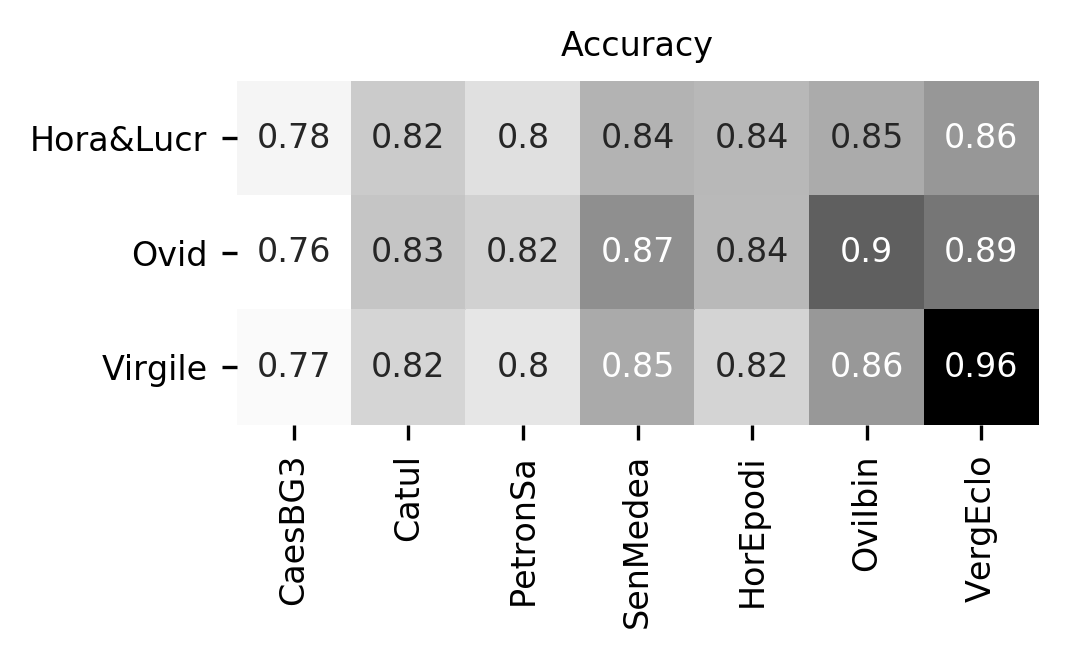
\includegraphics[width=1\linewidth]{figures/chap3/longreeVariante/LongreeVariante-AccuracyStyleDePoesie-Lemme.png}
    \end{minipage} \hfill
    \begin{minipage}[c]{0.55\linewidth}
        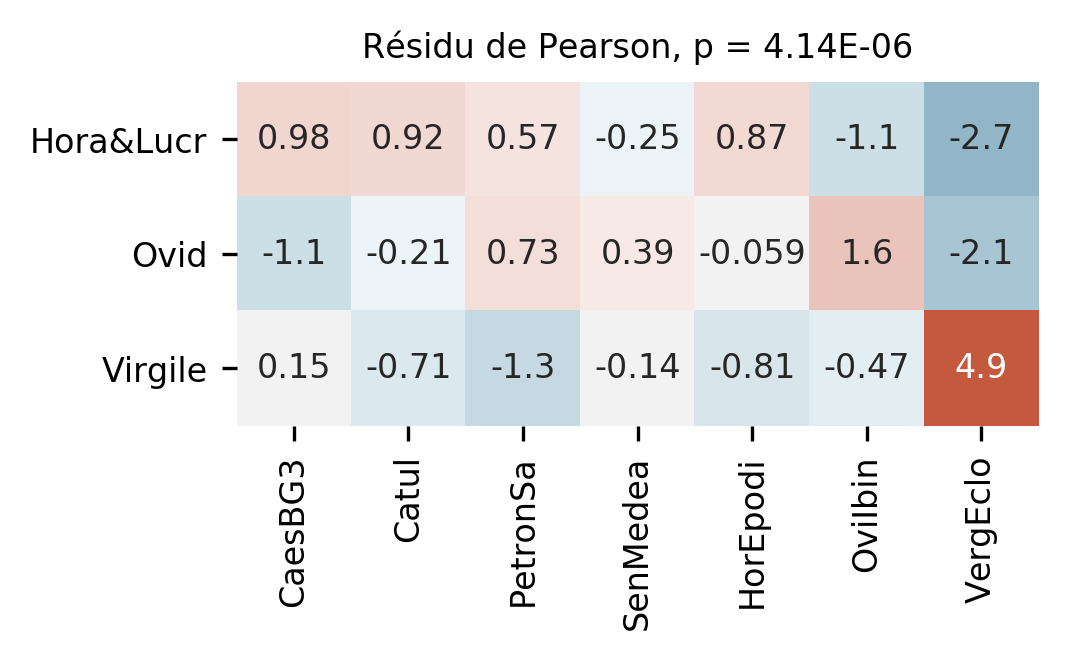
\includegraphics[width=1\linewidth]{figures/chap3/longreeVariante/LongreeVariante-AssocPlotStyleDePoesie-Lemme.png}
    \end{minipage}
    \caption{\textit{Accuracy} en lemme de modèles entraînés sur des poètes avec leurs résidus de Pearson}
    \label{fig:lemmatisation:longree:poetes}
\end{figure}

Les corpus d'entraînement des auteurs Virgile et Ovide ont un effet net (r=49 et r=1,6) sur les corpus de tests des auteurs respectifs. Si l'\textit{accuracy} de Virgile s'en ressent, celle d'Ovide reste globalement basse. Il faut rappeler ici la taille des corpus d'entraînement, seulement 90~000 tokens environ. Au contraire, le corpus mixte Horace et Lucrèce ne semble pas décoller, y compris sur les corpus d'Horace ou de Catulle. Les trois corpus n'ont pas une bonne reconnaissance du corpus prosaïque (César) ou semi-prosaïque (Pétrone). Bien que la \textit{Medea} de Sénèque soit mieux reconnue dans l'ensemble, le résidu de Pearson ne permet pas d'établir une forte corrélation avec un modèle en particulier.

\subsubsection{Style d'auteur, style de genre}

\begin{figure}[ht]
    \hspace*{-0.05\linewidth}
    \begin{minipage}[c]{0.55\linewidth}
        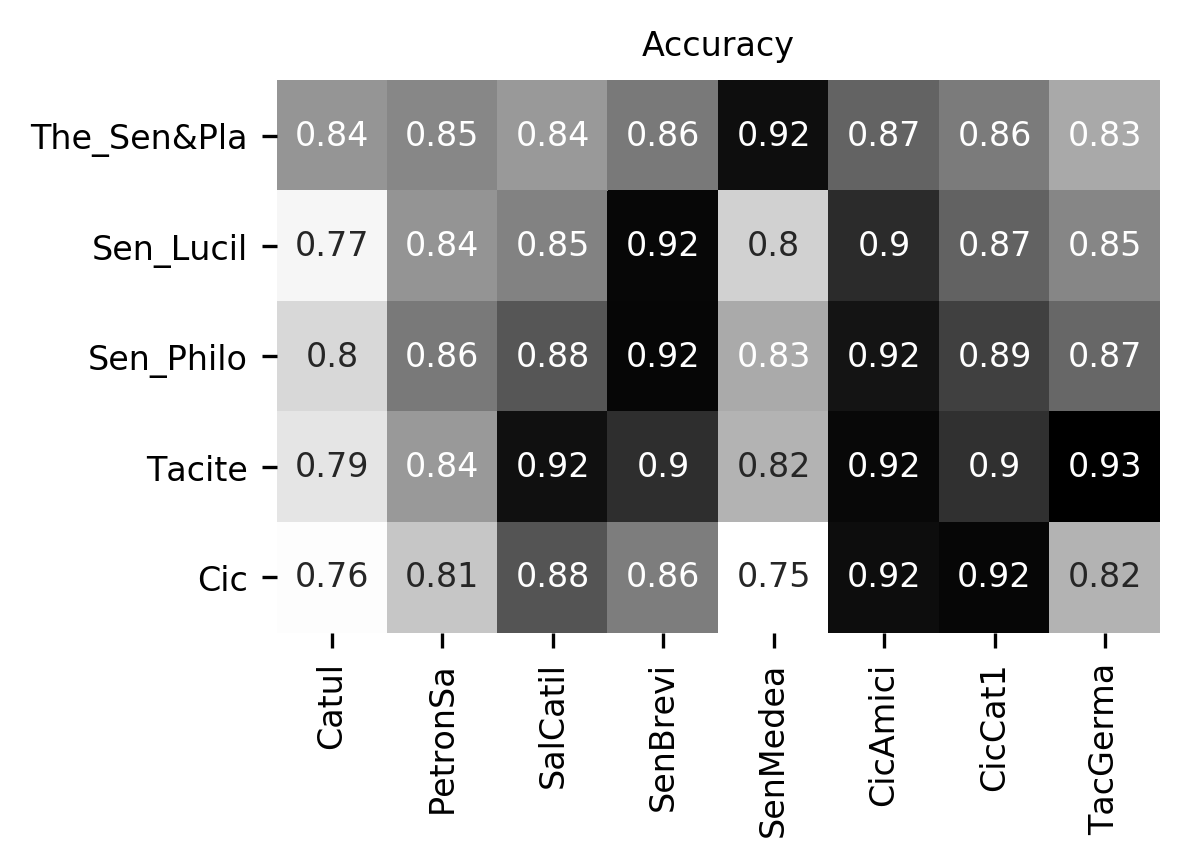
\includegraphics[width=1\linewidth]{figures/chap3/longreeVariante/LongreeVariante-AccuracyStyleDAuteurStyleDeGenre-Lemme.png}
    \end{minipage} \hfill
    \begin{minipage}[c]{0.55\linewidth}
        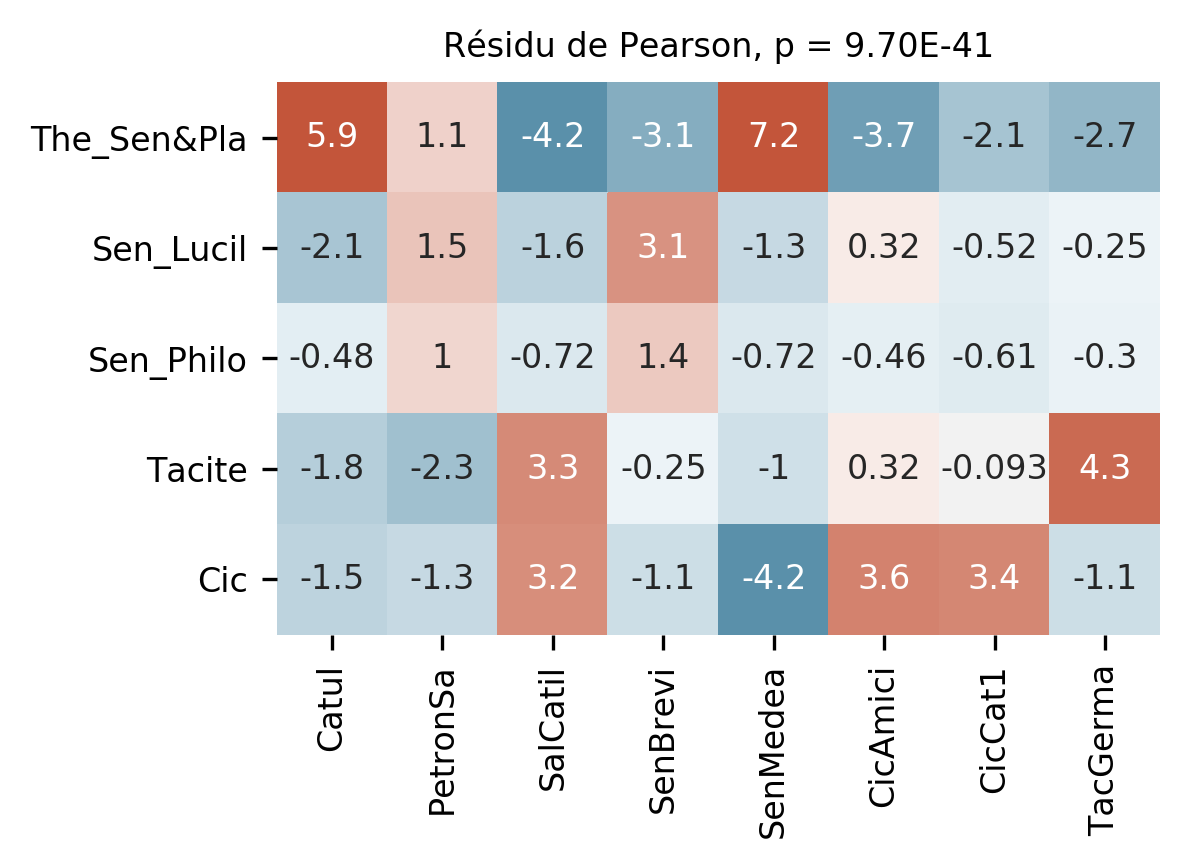
\includegraphics[width=1\linewidth]{figures/chap3/longreeVariante/LongreeVariante-AssocPlotStyleDAuteurStyleDeGenre-Lemme.png}
    \end{minipage}
    \caption{Accuracy en lemme de modèles avec leurs résidus de Pearson: les corpus d'entraînements ont été élaborés pour permettre d'identifier l'importance de l'auteur et du genre en termes de lemmatisation.}
    \label{fig:lemmatisation:longree:auteurVSforme}
\end{figure}

Dans cette étude, deux prosateurs font face à la prose de Sénèque sous deux formes (ses dialogues et traités d'une part, ses lettres d'autre part) et aux vers de Sénèque et de Plaute. On note tout de suite une nette relation entre accuracy et forme, puisque Sénèque a des R et des \textit{accuracies} particulièrement hauts sur Catulle et le théâtre de Sénèque. Au contraire, l'œuvre versifiée de Sénèque ne semble pas mieux comprendre le Sénèque prosaïque que d'autres prosateurs (résultats similaires entre Cicéron, \textit{De Amicitia}, \textit{In Catilinam} et le \textit{De Brevitate Vitae} de Sénèque). L'inverse est aussi remarqué puisqu'aucun des modèles de prose de Sénèque ne réagit nettement mieux que celui de Tacite, en \textit{accuracy} ou en résidu de Pearson. Les auteurs de proses fonctionnent bien sur eux-mêmes et Cicéron ainsi que Tacite fonctionnent particulièrement bien sur Salluste: on peut supposer que l'\textit{In Verrem} et les \textit{Philippicae} de Cicéron, formant le corpus d'entraînement ici, partagent avec Tacite et les \textit{In Catilinam} de Salluste des questions de pouvoir politique, de corruption et - par extension - un vocabulaire et un style assez proche. Au contraire, les œuvres philosophiques de Sénèque ne sont pas assez marquées, et en tout cas trop éloignées du \textit{De Amicitia} dans leur style pour influer de quelque manière. Pour finir, après deux tests, on se rend compte du caractère presque neutre du \textit{Satyricon} de Pétrone qui ne semble profiter ni de la prose ni du vers ni encore de la période, mais qui profite tout de même du passage de 90~000 à 115~000 tokens du corpus d'entraînement.

\subsubsection{Versificateur contre prosateur}

\begin{figure}[ht]
    \centering
    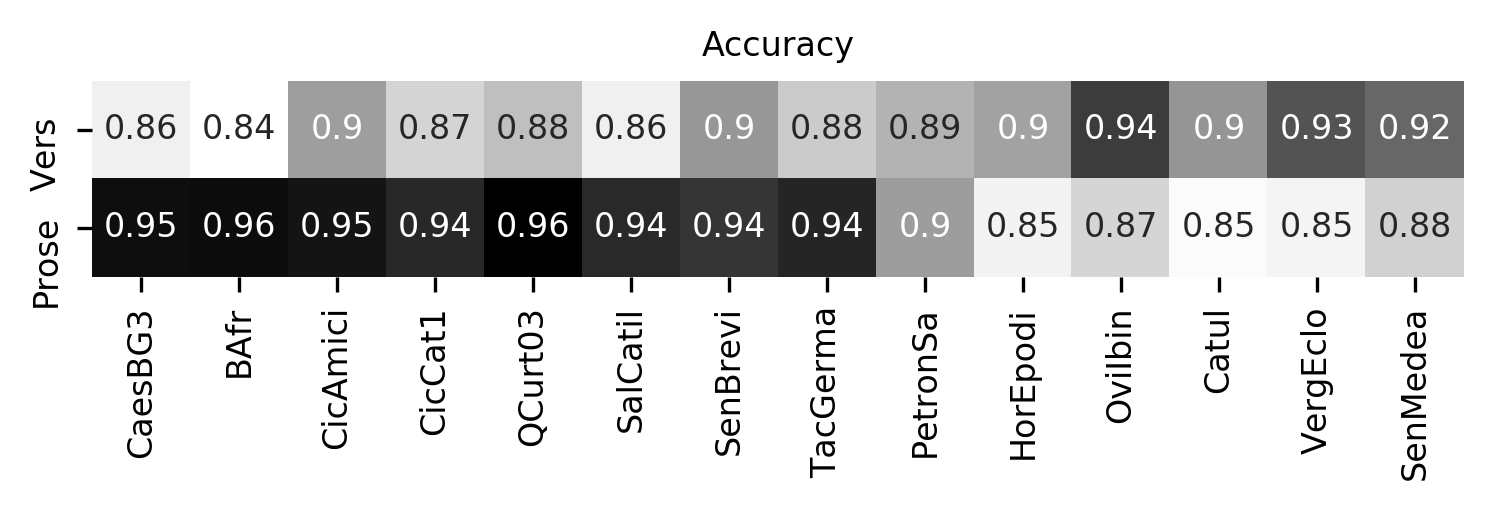
\includegraphics[width=0.7\linewidth]{figures/chap3/longreeVariante/LongreeVariante-AccuracyModeDExpression-Lemme.png}
    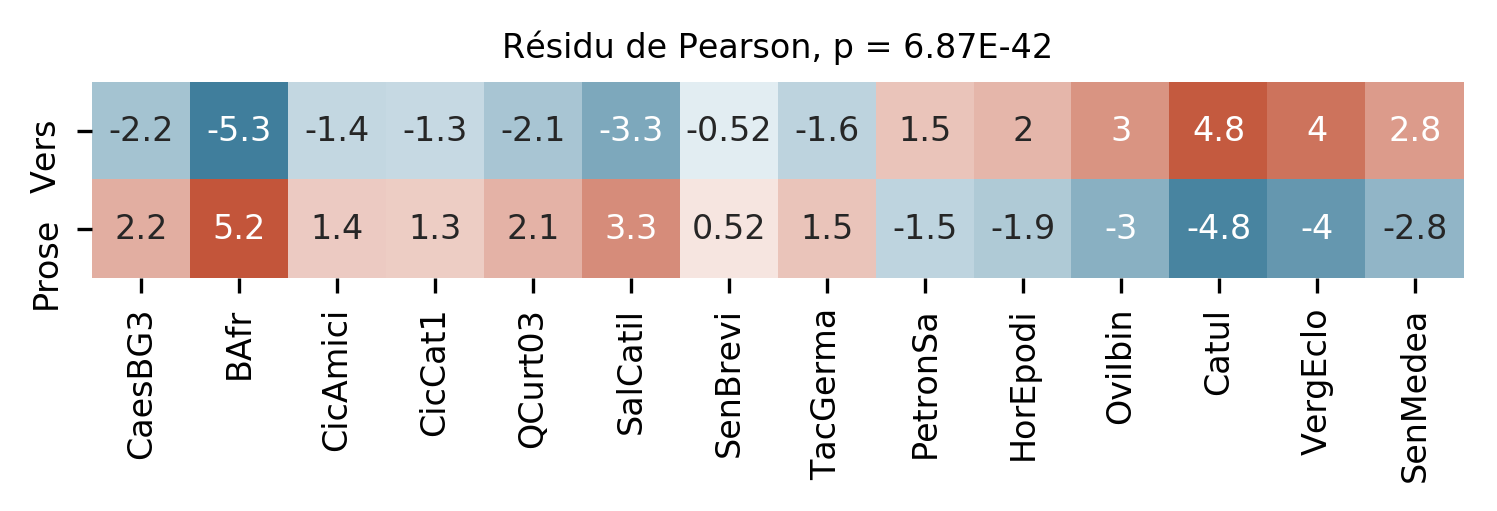
\includegraphics[width=0.7\linewidth]{figures/chap3/longreeVariante/LongreeVariante-AssocPlotModeDExpression-Lemme.png}
    \caption{\textit{Accuracy} en lemme de modèles avec leurs résidus de Pearson: chaque corpus est formé uniquement de prose ou de vers.}
    \label{fig:lemmatisation:longree:proseVSvers}
\end{figure}

Avec la troisième expérience, le corpus double en taille, mais présente désormais une unité de forme: celle d'un modèle en prose contre celle d'un modèle en vers. Les résultats sont nets, avec une très forte efficacité du modèle prose sur la prose, en $r$ ou en \textit{accuracy}, avec un écart allant jusqu'à 12~points pour le \textit{Bellum Africanum}. Ici, trois auteurs sont totalement absents  des corpus d'entraînement et doivent retenir notre attention, car, logiquement, le style d'auteur ne joue pas dans les scores: il s'agit de Pétrone, de Salluste et de Catulle (nous excluons le Pseudo-César du \textit{Bellum Africanum} par la proximité stylistique recherchée par l'auteur avec César). Nous notons que si la prose fonctionne bien mieux, les vers ne semblent pas nécessairement surperformer en \textit{accuracy} avec des écarts plus réduits, mais tout de même présents. Encore une fois, le \textit{Satyricon} fait office de frontière, avec l'écart le plus réduit de tout le corpus.

\subsubsection{Diversité des auteurs contre celle d'un auteur}

\begin{figure}[ht]
    \centering
    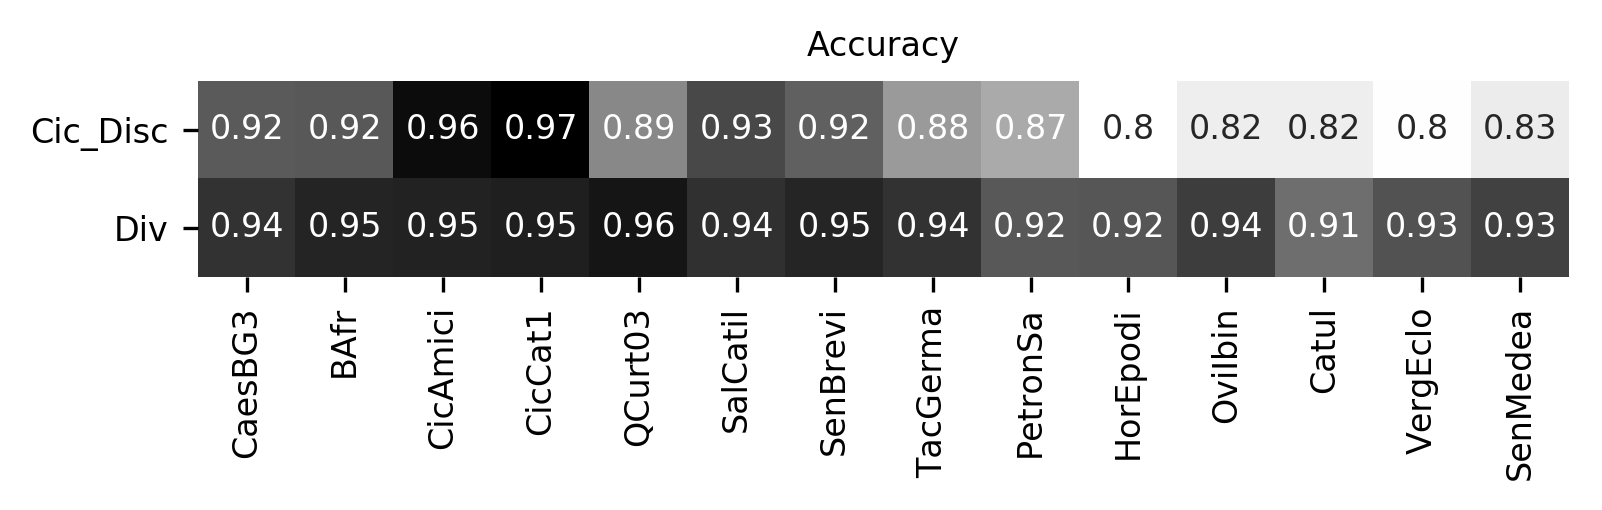
\includegraphics[width=0.7\linewidth]{figures/chap3/longreeVariante/LongreeVariante-AccuracyDiversiteDAuteursContreDiversiteDAuteur-Lemme.png}
    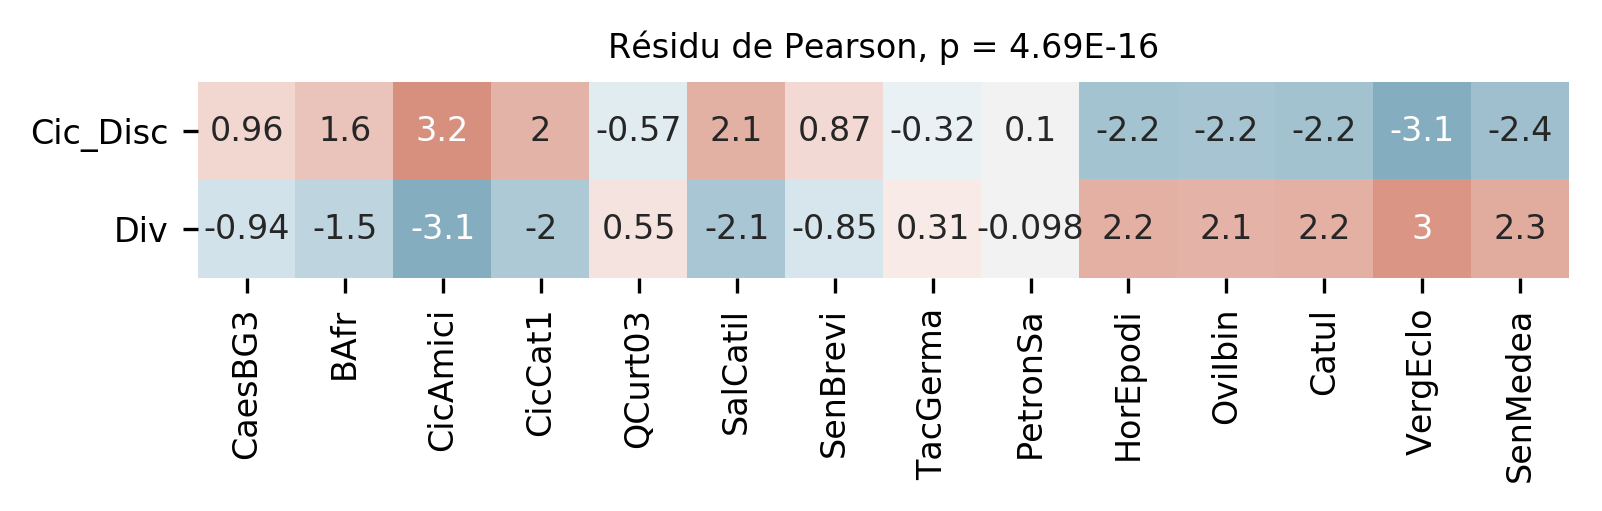
\includegraphics[width=0.7\linewidth]{figures/chap3/longreeVariante/LongreeVariante-AssocPlotDiversiteDAuteursContreDiversiteDAuteur-Lemme.png}
    \caption{Analyse de l'efficacité d'un grand corpus d'auteur contre une diversité de styles (\textit{Accuracy} en lemme et résidu de Pearson)}
    \label{fig:lemmatisation:longree:divAuteursVSTailleAuteur}
\end{figure}

Sur cette dernière expérience, nous posons la question suivante: dans le cadre d'un modèle entraîné sur un corpus déjà conséquent 390~000 tokens, la diversité des auteurs et des genres prime-t-elle sur celle d'un auteur ? Autrement dit, dans le cadre d'une création de corpus d'entraînement, vaut-il mieux annoter beaucoup d'auteurs, quitte à ne pas chercher à annoter les œuvres complètes, ou bien un seul ? Les résultats, en \textit{accuracy}, sont sans appel: la diversité des auteurs permet de surclasser un corpus uni-auteur sur tous les auteurs hors domaine (Salluste, Catulle, Pétrone), sur les auteurs partagés à l'exception de l'auteur utilisé dans le corpus unifié. Et nous noterons sur ce dernier corpus test que la différence est extrêmement limitée, de 0,01 à 0,02 points malgré une spécification du modèle sur le corpus cicéronien. Enfin, il semble que le \textit{Satyricon} fonctionne enfin mieux en \textit{accuracy} avec un mélange prose et vers, cependant, le $r$ ne nous permet pas de conclure en faveur de cette hypothèse.

\subsubsection{Conclusion}

Sur la base de ces résultats, on distingue les effets suivants:
\begin{itemize}
    \item Le style d'un auteur semble plus déterminant que l'époque de rédaction (figure \ref{fig:lemmatisation:longree:poetes}) ou la diversité en termes d'auteurs (figure \ref{fig:lemmatisation:longree:divAuteursVSTailleAuteur}), y compris quand ce style est copié par des imitateurs. Cet effet tend à se limiter sur des corpus très importants (figure \ref{fig:lemmatisation:longree:divAuteursVSTailleAuteur})
    \item La forme, en particulier poétique, prend le dessus sur le style d'un auteur (figures \ref{fig:lemmatisation:longree:auteurVSforme} et \ref{fig:lemmatisation:longree:proseVSvers}).
    \item La proximité de genre (philosophie, histoire en \ref{fig:lemmatisation:longree:auteurVSforme}) a un impact relativement faible. Mais, cet impact faible est à relativiser avec une possible proximité des thèmes des œuvres sélectionnées pour l'expérience..
\end{itemize}

\section{Modèle LASLA+ et étiquetage du corpus}

Après évaluation des limites du modèle sur le hors-domaine, puis des potentielles influences de composition des corpus d'entraînement, on entraîne un second modèle, \textit{LASLA+}, testé sur le même corpus de test, mais que l'on augmentera des corpus hors domaine ainsi que de la \textit{Vulgate} taguée par \textit{Proiel} alignée semi-automatiquement. Nous revenons alors sur les problèmes d'alignement de corpus, les probables erreurs qui se sont glissées et les difficultés que ce nouveau modèle rencontre. Nous aborderons ensuite la question du prétraitement (\textit{preprocessing}) et de son impact sur la lemmatisation pour finir sur une évaluation rapide du corpus annoté automatiquement, via la recherche de termes posant des problèmes dans le corpus qui nous intéresse.

\subsection{Modèle LASLA+ avec ajout des corpus et alignement de la \textit{Vulgate}}

Notre corpus LASLA ne présente aucun auteur tardif, et donc aucun auteur chrétien. Pour remédier à ce manque, un corpus latin tardif (mais non médiéval) existe et est libre de droits: celui de PROIEL\footcite{haug_creating_2008}. Proiel propose trois textes qui ne font pas partie du corpus LASLA, à savoir la \textit{Vulgate} de Jérôme, le \textit{Peregrinatio Aetheriae} et enfin l'\textit{Opus agriculturae} de Palladius. Pour des raisons de temps et d'optimisation de ce dernier, seule la Vulgate a été alignée avec le corpus du LASLA.

On pourrait penser qu'un alignement d'un modèle à l'autre est une tâche simple, d'autant qu'\textit{a priori} le LASLA découpe rarement les lemmes en fonction de leur sens, mais uniquement en fonction de leur POS et leur genre\footnote{On note tout de même \textit{populus1}, le peuple, et \textit{populus2} parmi les exceptions.}. Cependant, un alignement lemma/POS/morphologie requiert de s'assurer que les deux corpus ont le même usage de la morphologie et dans une moindre mesure des POS. Pour les lemmes, l'alignement se fait dans l'ordre suivant:
\begin{enumerate}
    \item Le lemme est présent tel quel dans le dictionnaire du LASLA. L'annotation lemme est donc conservée.
    \item Le lemme existe avec un seul indice de désambiguïsation: il est aligné
    \item Le lemme existe avec plusieurs indices de désambiguïsation, on compare alors les POS, par exemple pour \textit{ad} entre ADV et PRE.
    \item Dans le cas où le lemme ne rentre pas dans ces catégories, on vérifie qu'il n'existe pas sous une autre orthographe, par exemple \textit{adulescens} chez Proiel existe sous \textit{adolescens1} ou \textit{adolescens2} suivant la POS, \textit{excaedo} en \textit{excido1}.
\end{enumerate}

La morphologie nécessite par ailleurs un alignement via la suppression du genre pour les formes qui ne sont ni des adjectifs, ni des pronoms, ni des participes. Ensuite, les genres sont alignés via la déclinaison dont relèvent les adjectifs ou les formes. La morphologie est aussi complétée: les indéclinables ne sont pas analysés ainsi par Proiel (mais plutôt comme des absences de morphologie), ce qui nécessite un réalignement. On finit par normaliser l'orthographe des formes et lemmes pour les couples U/V et J/I puis une première conversion est faite. Si cette étape est itérative, l'objectif reste de réduire au maximum les lemmes à corriger manuellement. Enfin, sur les derniers lemmes, plusieurs centaines, on aligne à la main avec le référentiel du LASLA et on crée des entrées quand le lemme est absent, ce qui est souvent le cas pour les noms propres. Cette dernière catégorie est très importante et démontra une nouvelle difficulté pour l'apprentissage, avec des cas d'hapax comme cette généalogie de \textit{Luc}, 3.23:

\begin{quote}
\blockquote{\textit{Et ipse Jesus erat incipiens quasi annorum triginta, ut putabatur, filius Joseph, qui  \\fuit Heli, qui fuit Mathat, \\
qui fuit Levi, qui fuit Melchi, qui fuit Janne, qui fuit Joseph, \\
qui fuit Mathathiæ, qui fuit Amos, qui fuit Nahum, qui fuit Hesli, qui fuit Nagge, \\
qui fuit Mahath, qui fuit Mathathiæ, qui fuit Semei, qui fuit Joseph, qui fuit Juda, \\
qui fuit Joanna, qui fuit Resa, qui fuit Zorobabel, qui fuit Salatheil, qui fuit Neri, \\
\textit{...} \\
qui fuit Sarug, qui fuit Ragau, qui fuit Phaleg, qui fuit Heber, qui fuit Sale, \\
qui fuit Cainan, qui fuit Arphaxad, qui fuit Sem, qui fuit Noë, qui fuit Lamech, \\
qui fuit Methusale, qui fuit Henoch, qui fuit Jared, qui fuit Malaleel, qui fuit Cainan, \\
qui fuit Henos, qui fuit Seth, qui fuit Adam, qui fuit Dei.}}
\end{quote}

Cette présence d'hapax pose un double problème dans la mesure où l'orthographe hébraïque ne se fixe pas par usage, telle \textit{Sarug/Seruch}, ou des formes qui n'existent dans le \textit{Forcellini} ou son appendice \textit{Onomasticon} que dans le corps du texte, tel \textit{Azor}, présent dans l'entrée \textit{Sadoc}.

Après cet alignement, on ajoute les données des \textit{Priapea} et du corpus chrétien, nous permettant d'obtenir une plus grande diversité de textes et une plus grande couverture thématique et temporelle et donc lexicale. L'entraînement de ce nouveau modèle obtient un score très légèrement moins bon que le corpus d'origine (\textit{cf.} table \textbf{A AJOUTER}). Il est probable que l'ajout de données dont l'édition n'a pas été traitée de la même manière que les autres données du corpus du LASLA ajoute du bruit: c'est finalement une bonne chose, car cette variété permet aussi de s'éloigner d'un corpus \enquote{parfait} et de se rapprocher \textit{de facto} du corpus que l'on traitera ensuite sur lequel l'intervention humaine, au niveau de la segmentation syntaxique, est minimale.

\subsection{Importance du \textit{pre-processing}}

Nous avons parlé jusque là principalement des méthodes d'entraînement et de l'algorithme responsable de la lemmatisation. Il peut exister un certain nombre de problèmes lorsque l'on passe d'une application sur données éditées - tokenisées à la main au niveau phrase et mot, harmonisées en orthographe, etc. - à des données \textit{in situ}. Cette problématique a déjà été étudiée sur d'autres types de tâches comme la classification de textes\footcite{camacho-collados_role_2018} et montre en général des conséquences - au pire mineures - en termes de résultats. Or, nous avons vu que les données du corpus LASLA possèdent une très forte éditorialisation, allant des normalisations de couple u/v et j/i à l'absence de ponctuation, qui, dans le cas d'une lemmatisation \textit{in situ}, influencerait probablement la lemmatisation. En effet, dans la phase de transcodage de \textit{pie}, toute lettre inconnue - comme v par exemple - est codée \textit{de facto} en tant que lettre inconnue et non en tant que v, puisqu'elle n'a pas pu avoir de représentation apprise dans l'espace de projection des caractères. Il faut donc s'assurer que ces lettres, lorsqu'une alternative est possible, sont traduites, remplacées. Du côté de la ponctuation, le choix est tout autre: il faut pouvoir s'appuyer sur la ponctuation pour les tâches telles que la reconnaissance des phrases ou celles des abréviations, mais s'assurer qu'elles disparaissent pour la phase de lemmatisation pure puis réapparaissent pour les futures étapes de notre recherche. D'autres cas, comme la présence de formes grecques ou de nombres, sont indiqués et simplifiés afin d'éviter au lemmatiseur d'apprendre à lemmatiser le grec ainsi que les chiffres romains en chiffres arabes, chose faisable par un programme simple, car extrêmement régulé, mais plus difficile pour un réseau neuronal avec très peu d'exemples.

\begin{table}[ht]
    \centering
    \resizebox{\linewidth}{!}{%
    \begin{tabular}{l|rrrr}
    \hline
                                              & A                 & B                 & C              & D              \\ \hline
    Normalisation des lettres                 & Non               & Oui               & Non            & Oui            \\
    Suppression des formes inconnues (points) & Non               & Non               & Non            & Oui            \\
    Tokenisation Phrase                       & Ponctuation Forte & Ponctuation Forte & 35 Mots        & 35 Mots        \\ \hline
    lemma              & \textbf{-1,51} & -0,22          & \textbf{-1,62} & -0,23 \\
    Deg                & -0,30          & -0,16          & -0,26          & -0,06 \\
    Numb               & -0,41          & -0,31          & \textbf{-0,56}          & -0,12 \\
    Person             & -0,05          & 0,00           & -0,06          & -0,03 \\
    Mood\_Tense\_Voice & -0,11          & -0,02          & -0,12          & -0,04 \\
    Case               & \textbf{-0,76} & \textbf{-0,66} & \textbf{-1,41} & \textbf{-0,32} \\
    Gend               & -0,28          & -0,13          & -0,23          & -0,11 \\
    pos                & \textbf{-0,57} & -0,33          & \textbf{-0,66} & -0,18 \\ \hline
    \end{tabular}}
    \caption{Impact de la normalisation sur l'\textit{accuracy}, en \%.}
    \label{tab:lemmatisation:normalisation}
\end{table}

Dans ce cadre, on propose une expérience assez simple: à partir des données de latin tardif, qui contiennent une orthographe \textit{in situ} et une ponctuation, on fait varier le contenu à lemmatiser en fonction de trois variantes combinables:
\begin{itemize}
    \item Une normalisation des lettres et formes, principalement u/v et j/i,
    \item Une suppression pour l'étape de lemmatisation de la ponctuation et des formes inconnues comme le grec,
    \item Une tokenisation du texte sur la base de la ponctuation forte (points, guillemets, parenthèses, etc.) ou sur une fenêtre de 35 mots. Cette fenêtre est la fenêtre proposée par défaut par \textit{pie}. Plusieurs fenêtres raisonnables (multiples de 5 jusqu'à 35) ont été testées ici, mais elles présentaient des résultats dans des marges minimales.
\end{itemize}
Les résultats, visibles en table \ref{tab:lemmatisation:normalisation}, montrent un fort impact de la conservation des signes de ponctuation et des lettres inconnues avec des scores baissant de 1,51\% à 1,62\% quand les deux sont ignorés. Il faut noter que la conservation des lettres inconnues a - semble-t-il - un impact assez limité (-0,22\%). Au niveau des tâches auxiliaires, toutes les tâches sont touchées sauf la reconnaissance de personne, le cas et la POS étant particulièrement influencées avec des baisses allant jusqu'à -0,76\%. Dans le cadre où la tokenisation des phrases est faite tous les 35 mots, la lemmatisation, le cas et la POS sont légèrement influencées aux alentours de -0,20\%. On note ici que l'accumulation de bruit n'est pas de l'ordre de l'addition: plus le nombre de régularisations manquantes croît, plus les tâches sont influencées. Si les signes de ponctuations ont été supprimés des calculs d'\textit{accuracy} dans l'expérience précédente, nous pouvons retrouver aussi les bizarreries que crée la lemmatisation de signes totalement inconnus tels que dans l'\textit{incipit} de la \textit{Bellum Gallicum} (cf. \textit{infra}). Dans une telle situation, il est clair que le prétraitement est inséparable d'une bonne lemmatisation via des réseaux neuronaux.

\begin{quote}
    \textbf{Source}\\
    \blockquote{Gallia omnis divisa in partes tres , quarum unam incolunt Belgae , aliam Aquitani tertiam , qui ipsorum lingua Celtae nostra Galli appellantur.}\\
    \textbf{Lemmatisation brute}\\
    \blockquote{gallia omnis \textbf{dico} in pars tres \textbf{qvi} qvi vnvs incolo belgae \textbf{vnde} alivs aqvitani tertivs \textbf{vi} qvi ipse lingva celtae noster galli appello \textbf{nonvs}}\\
    \textbf{Lemmatisation avec normalisation}\\
    \blockquote{gallia omnis divido in pars tres , qvi vnvs incolo belgae , alivs aqvitani tertivs , qvi ipse lingva celtae noster galli appello .}\\
    
    Exemple de bruit causé dans la lemmatisation lorsqu’ aucun prétraitement n'est effectué. En gras les erreurs introduites par la lemmatisation: on remarque qu'en dehors de la lemmatisation des points qui est totalement erronée, \textit{divisa} est aussi mal analysé, certainement à cause du bruit de ponctuation et de la lettre v.
    \label{quote:lemmatisation:gallia-errors}
\end{quote}


%\subsection{Étiquetage du corpus: exploration et différences entre le modèle LASLA et le modèle LASLA+}
 
%Dans cette section, nous ne proposons pas une étude aussi poussée que celles en, \ref{subsec:lemmatisation:hors-domaine} mais une analyse rapide des différences de résultats sur quelques termes qui ont montré des limites pour nos modèles.
\clearpage
\section*{Conclusion}

Entre les premiers concordanciers et la mécanisation de leur production, sept siècles se sont écoulés. En revanche, le concordancier aura ensuite été rapidement dépassé. L'évolution technologique résultant de l'informatisation d'abord, de sa démocratisation croissante et de la progression exponentielle des puissances de calculs a permis d'aborder les textes latins sous de nouveaux angles: celui du quantitatif linguistique d'abord, et celui de l'annotation automatique ensuite.

Dans les années 1960, il serait présomptueux de voir dans le travail du LASLA autre chose qu'une approche systématique de la linguistique latine, déjà bien suffisante pour l'époque. Cette ambition, qui dépasse le cas d'un seul auteur, a permis en une soixantaine d'années de couvrir une part importante du corpus classique. Tout en assurant un équilibre et une variété inégalée dans les genres et auteurs représentés, ce corpus a atteint plus d'un million et demi de mots hors ponctuation. Ce travail a pu nourrir des travaux quantitatifs des équipes du laboratoire producteur des données, mais aussi faire naître des collaborations avec d'autres, comme pour le lancement d'Hyperbase à Nice.

Mais c'est bien l'ouverture des données du LASLA qui a changé radicalement le paysage de la lemmatisation latine. En novembre 2018, lors de l'atelier international \textit{Text Encoding: Latinists looking for new synergies} organisé au LASLA, Dominique Longrée et Margerita Fantoli convient différents acteurs des humanités numériques latines (membres de l'ERC LILA, Bridget Almas d'Alpheios, Philipp Roelli de \textit{Corpus Corporum}, etc.). Cette ouverture et cet événement ont eu des répercussions sans précédents dans le champ d'étude. Plusieurs institutions, toutes avec leurs propres objectifs et approches des corpus, ont alors à leur disposition le plus grand corpus de latin classique intégralement annoté.

Sans cet apport, le travail présenté ici n'aurait probablement pas connu les mêmes succès. Les tests sur les lemmatiseurs connus, à partir des corpus limités de \textit{Perseus} ou de \textit{Proiel}, ne présentaient alors pas une qualité suffisante d'annotation pour traiter en intégralité notre corpus massif. Nous ne pouvons que souligner l'importance qu'a cette ouverture de données pour l'ensemble du champs. En dehors même de la question de la performance technique de nouveaux modèles, cette lemmatisation va permettre d'améliorer substantivement la recherche dans de larges bases.

La lemmatisation et l'annotation morpho-syntaxe automatiques du latin sont-elles pour autant des questions résolues ? La réponse est bien évidemment négative, et il est désormais temps de se tourner vers la production de nouveau corpus d'entraînement, vers d'autres périodes ou d'autres genres. Avec l'ouverture du corpus du LASLA, nous avons désormais un exemple sur lequel nous appuyé pour augmenter le corpus. Le corpus d'Anthony Glaise\footcite{glaise_2020_corpus_tardif} que nous avons co-construit est un premier pas dans cette direction: l'inclusion prévue de la \textit{Legenda Aurea}, et donc de l'époque médiévale, et celle de l'\textit{Utopia} de Thomas More, et donc de l'époque moderne, sont des premières incursions pour vérifier la résistance du modèle à d'autres périodes. La deuxième étape concerne la lemmatisation et l'annotation morpho-syntaxique d'un nombre grandissant de ressources non normalisées suivant les mêmes standards que le corpus LASLA+, qu'il s'agisse de données épigraphiques pour l'Antiquité ou bien de documents de la pratique pour le Moyen-Âge.
